\subsubsection{Reference architecture}
\label{sec:reference_archi}
%\GB{a good start is the paper from Casado et al., published at PRESTO'10, where the idea of a network hypervisor is introduced. A quick introduction of network virtualization in general, and how SDN stands in this landscape, would be helpful. Please refer to the following website: \url{http://packetpushers.net/sdn-network-virtualization-hypervisors/}. I suggest to even go as far as to mention the state of the art of network virtualization: from VLANs and VPNs, to network slicing, to network hypervisors}
A reference architecture is the theoretical design of an element that will include all necessary components. 
We consider here the design of a network hypervisor supporting a secure virtual network migration.
A network hypervisor should support the following operations:
\begin{itemize}
    \item Providing an abstraction of the physical infrastructure to tenants
    \item Providing an interface for tenants to interact with their virtual network
    \item Ensuring isolation between tenants to prevent unwanted interactions 
    \item Enabling automated virtual network migration in case of attacks or failures
    \item Ensuring security of the hypervisor and the virtual networks
\end{itemize}


\begin{figure}[ht]
\centering



\tikzset{every picture/.style={line width=0.75pt}} %set default line width to 0.75pt        

\begin{tikzpicture}[x=0.75pt,y=0.75pt,yscale=-1,xscale=1]
%uncomment if require: \path (0,587.1666717529297); %set diagram left start at 0, and has height of 587.1666717529297

%Rounded Rect [id:dp6657423098815228] 
\draw  [fill={rgb, 255:red, 184; green, 233; blue, 134 }  ,fill opacity=1 ] (54,393.93) .. controls (54,371.51) and (72.18,353.33) .. (94.6,353.33) -- (401.4,353.33) .. controls (423.82,353.33) and (442,371.51) .. (442,393.93) -- (442,515.73) .. controls (442,538.16) and (423.82,556.33) .. (401.4,556.33) -- (94.6,556.33) .. controls (72.18,556.33) and (54,538.16) .. (54,515.73) -- cycle ;
%Straight Lines [id:da9581441235133058] 
\draw    (139,461.33) -- (233,415) ;


%Straight Lines [id:da390156809167017] 
\draw    (254,527.33) -- (348,481) ;


%Straight Lines [id:da016159254093403685] 
\draw    (256,411.33) -- (360,463.33) ;


%Straight Lines [id:da1558560515309626] 
\draw    (139,470.33) -- (243,522.33) ;


%Image [id:dp1943708609890895] 
\draw (248,527.83) node  {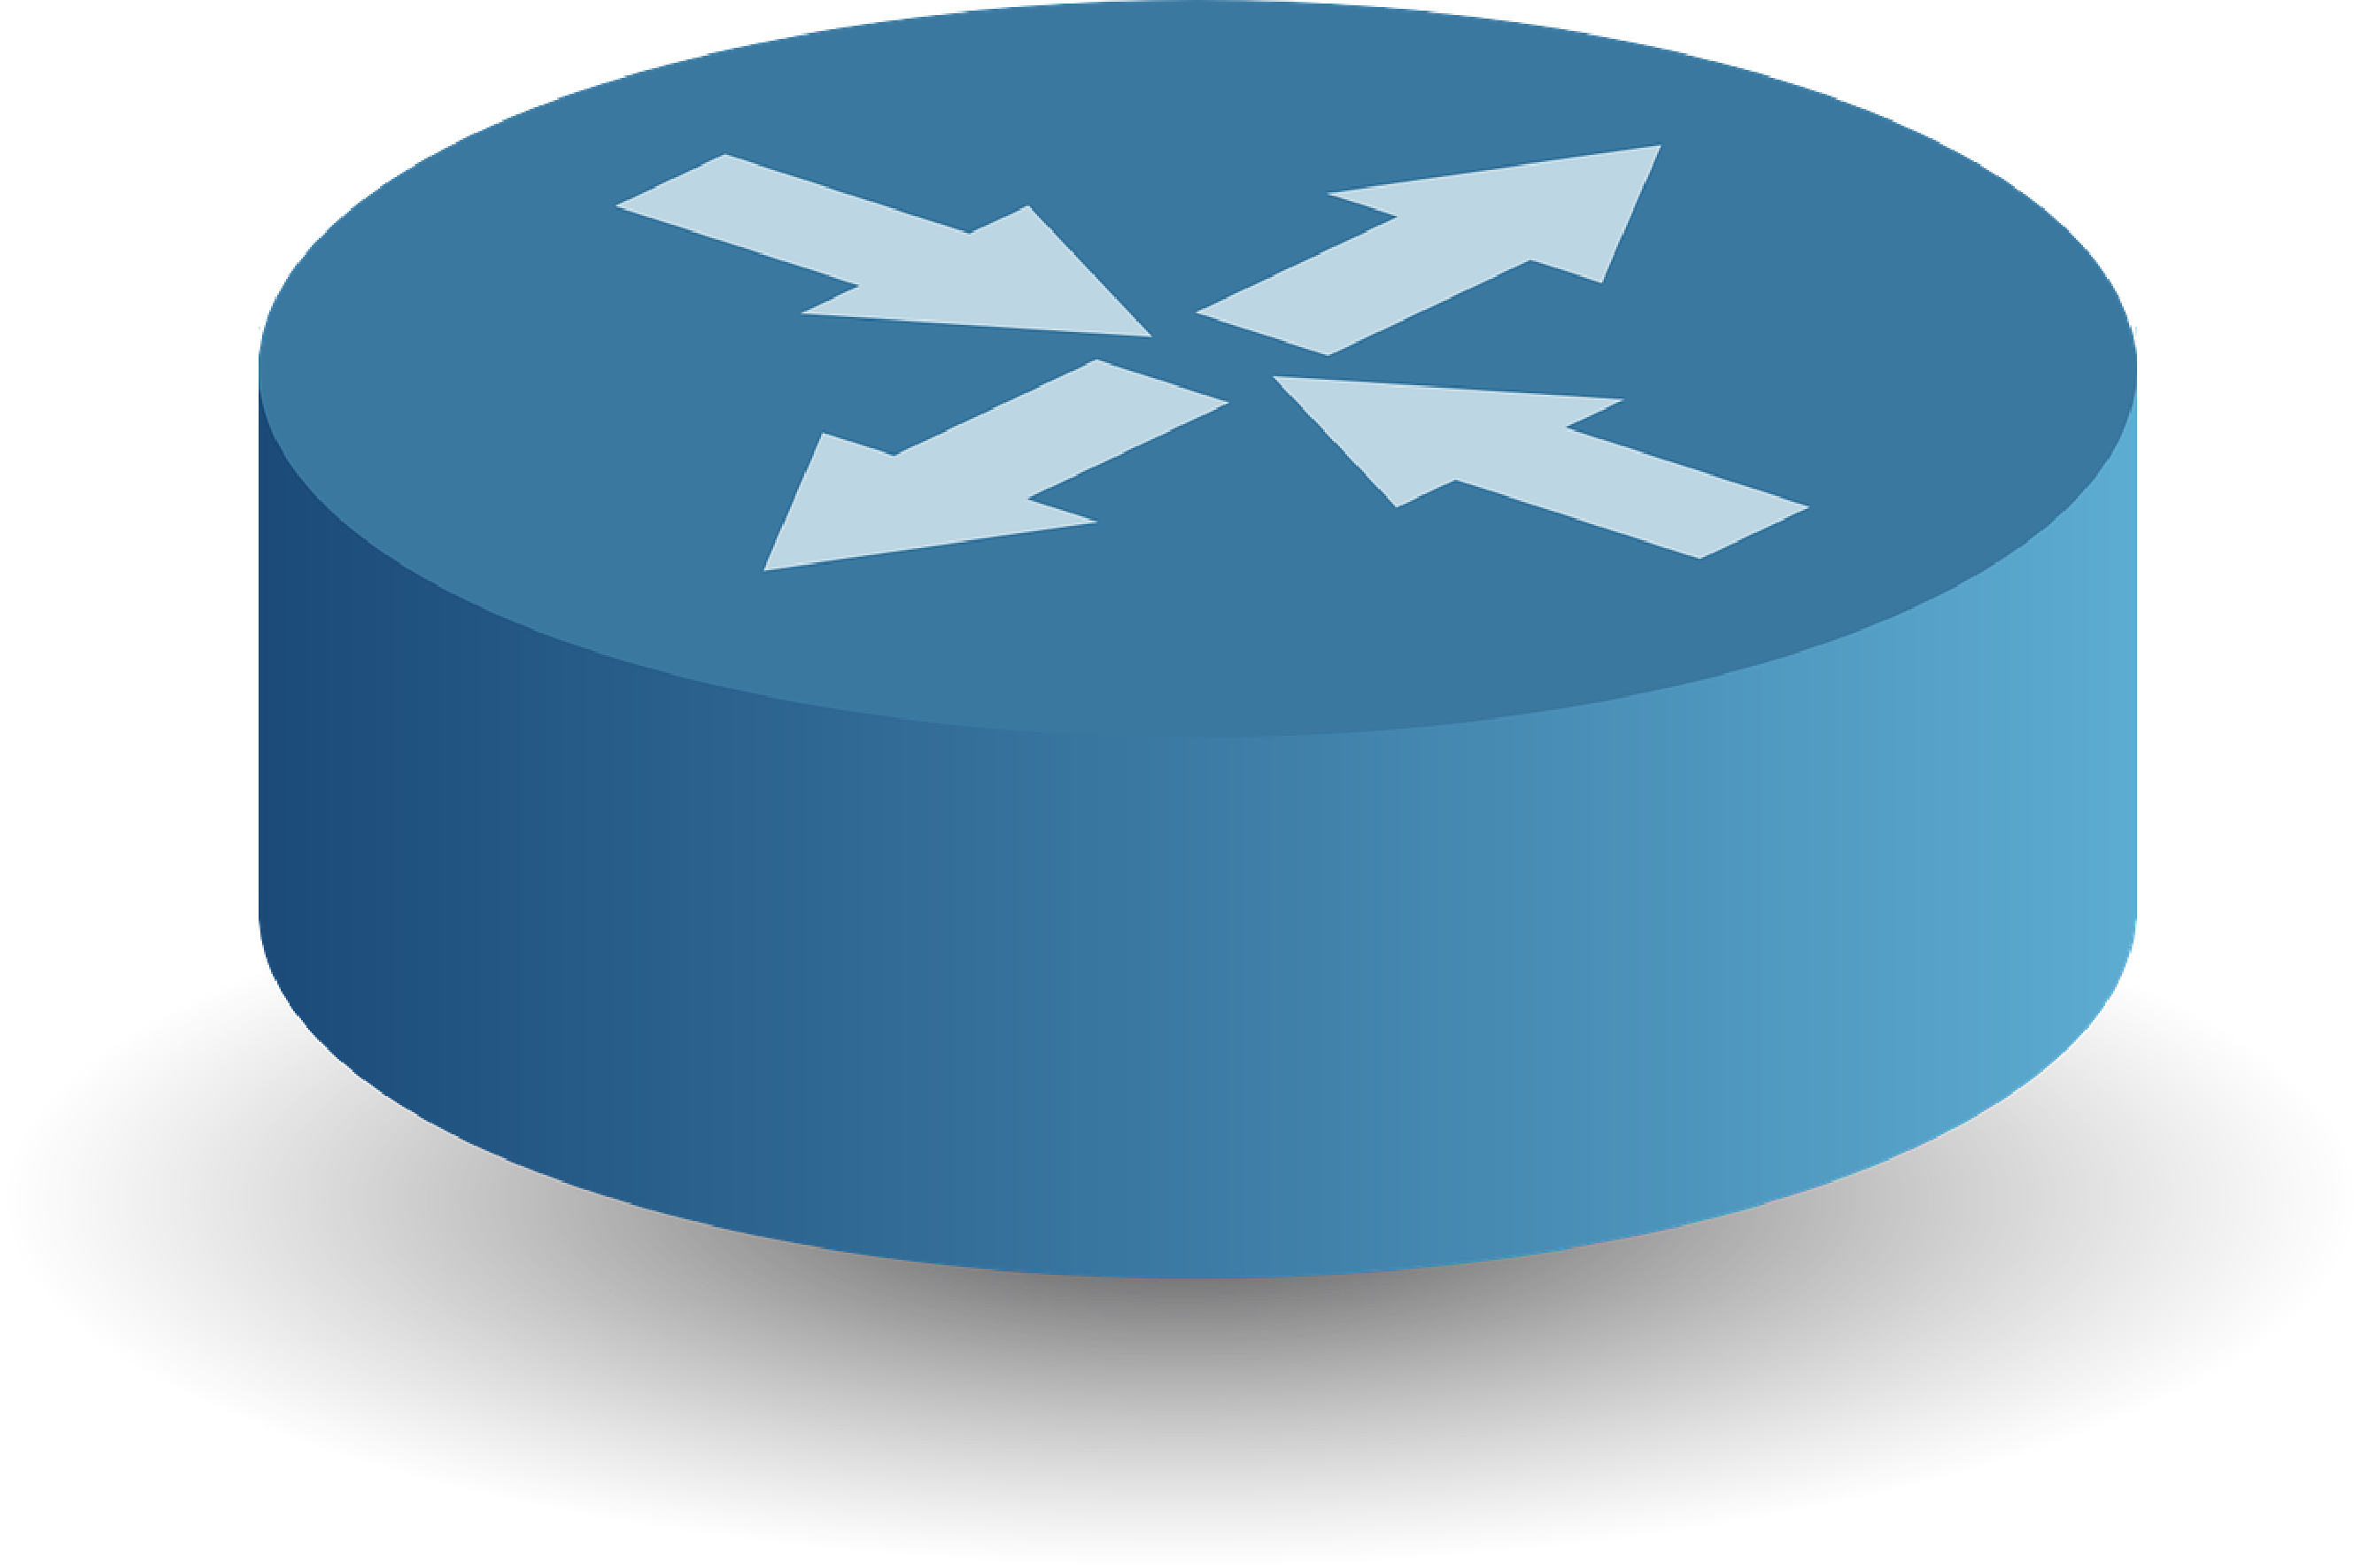
\includegraphics[width=52.5pt,height=52.5pt]{figures/router-29825_1280.pdf}};
%Image [id:dp4786061414756648] 
\draw (248,407.83) node  {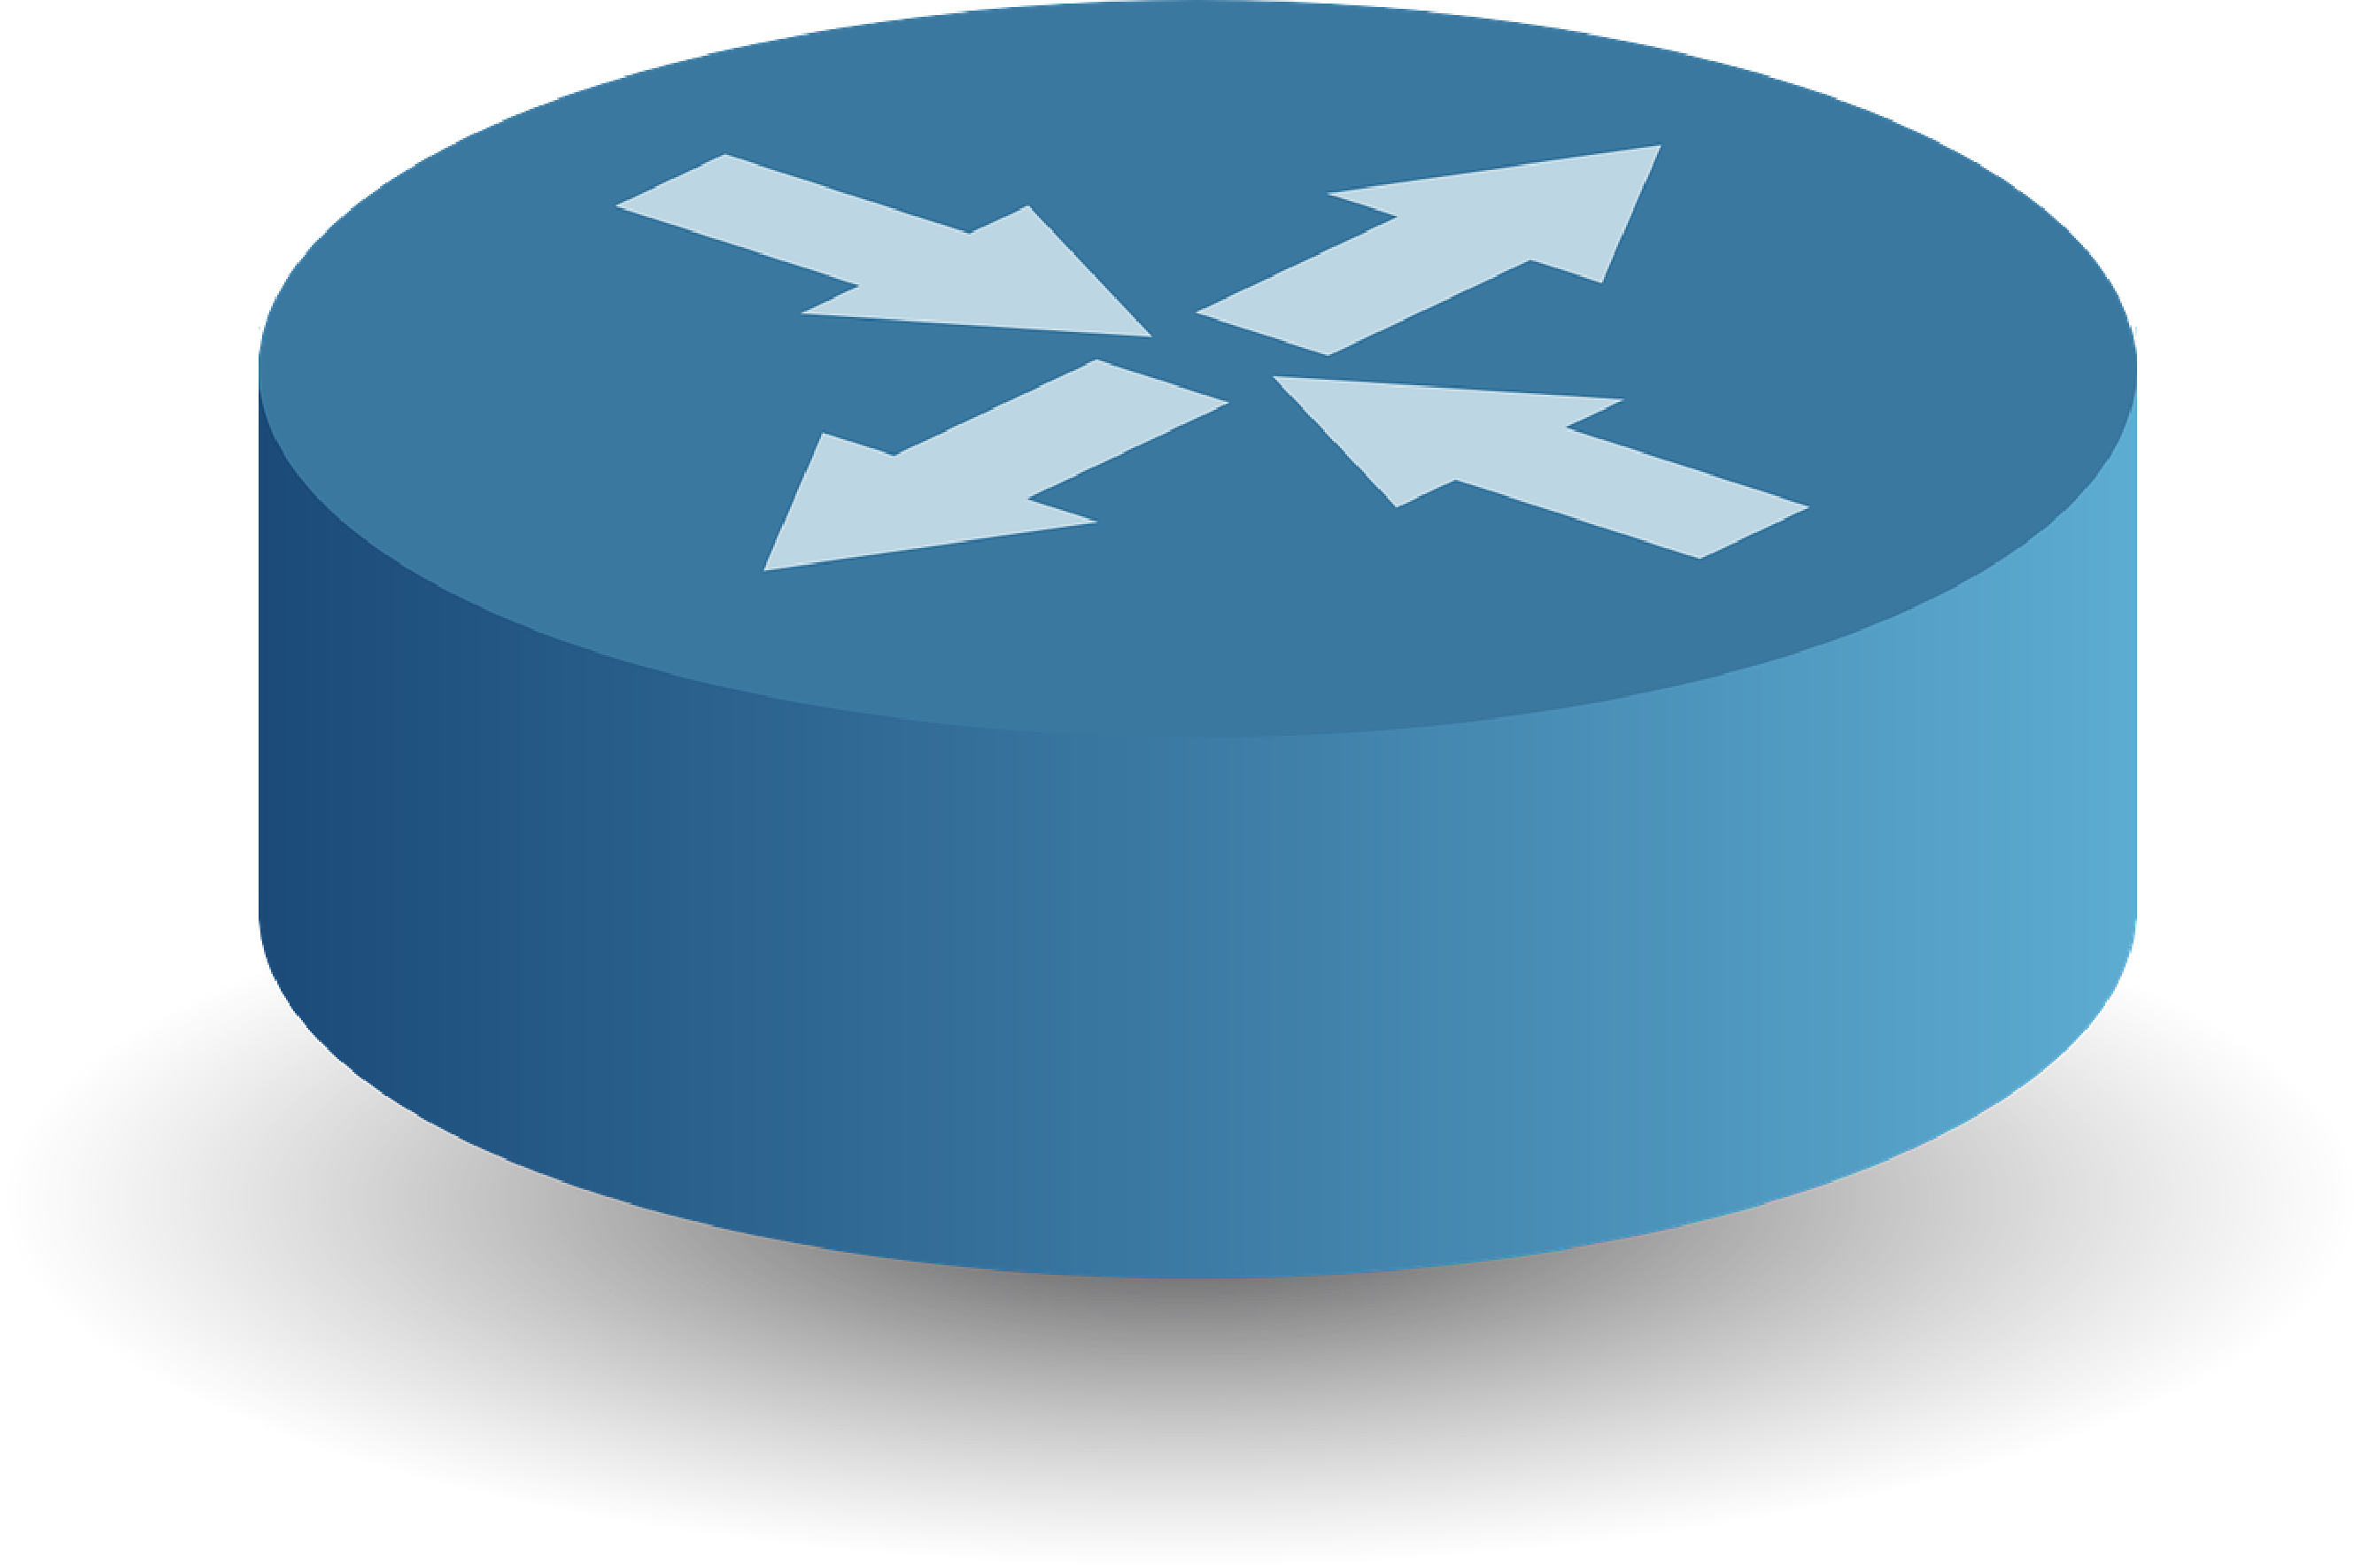
\includegraphics[width=52.5pt,height=52.5pt]{figures/router-29825_1280.pdf}};

%Image [id:dp9691436731399989] 
\draw (365.5,467.83) node  {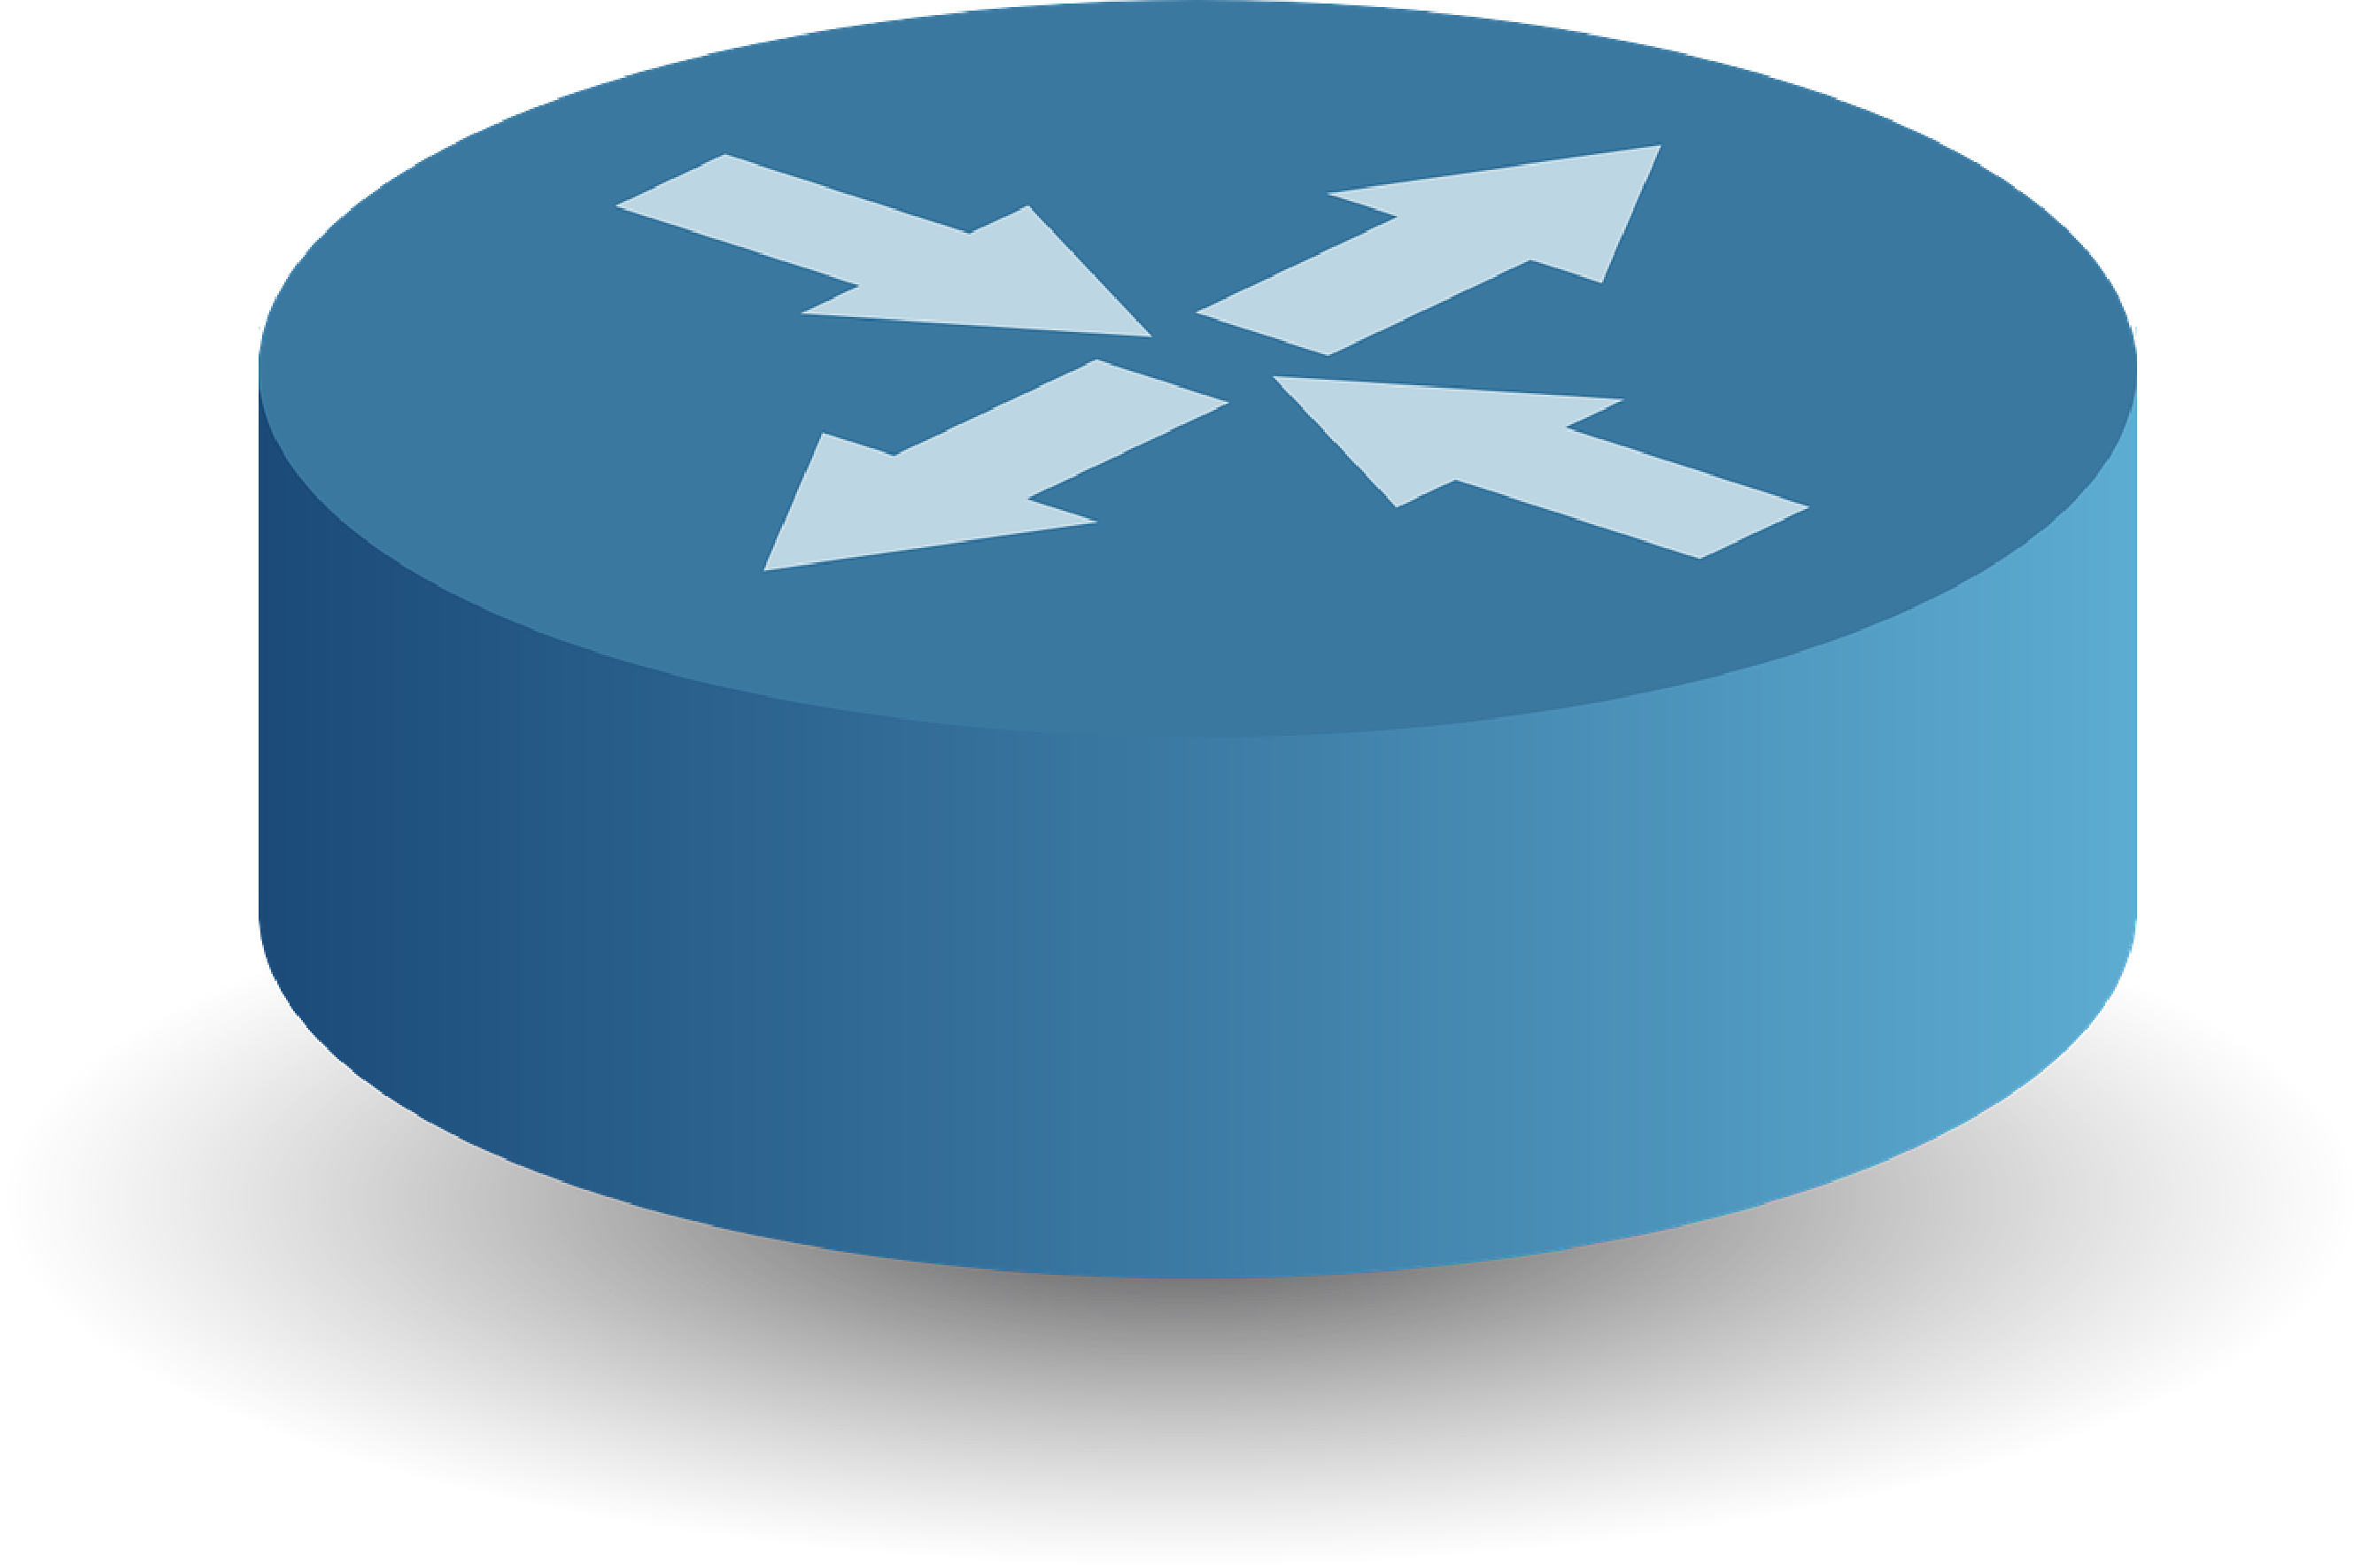
\includegraphics[width=52.5pt,height=52.5pt]{figures/router-29825_1280.pdf}};
%Image [id:dp9494715890151124] 
\draw (130.5,467.83) node  {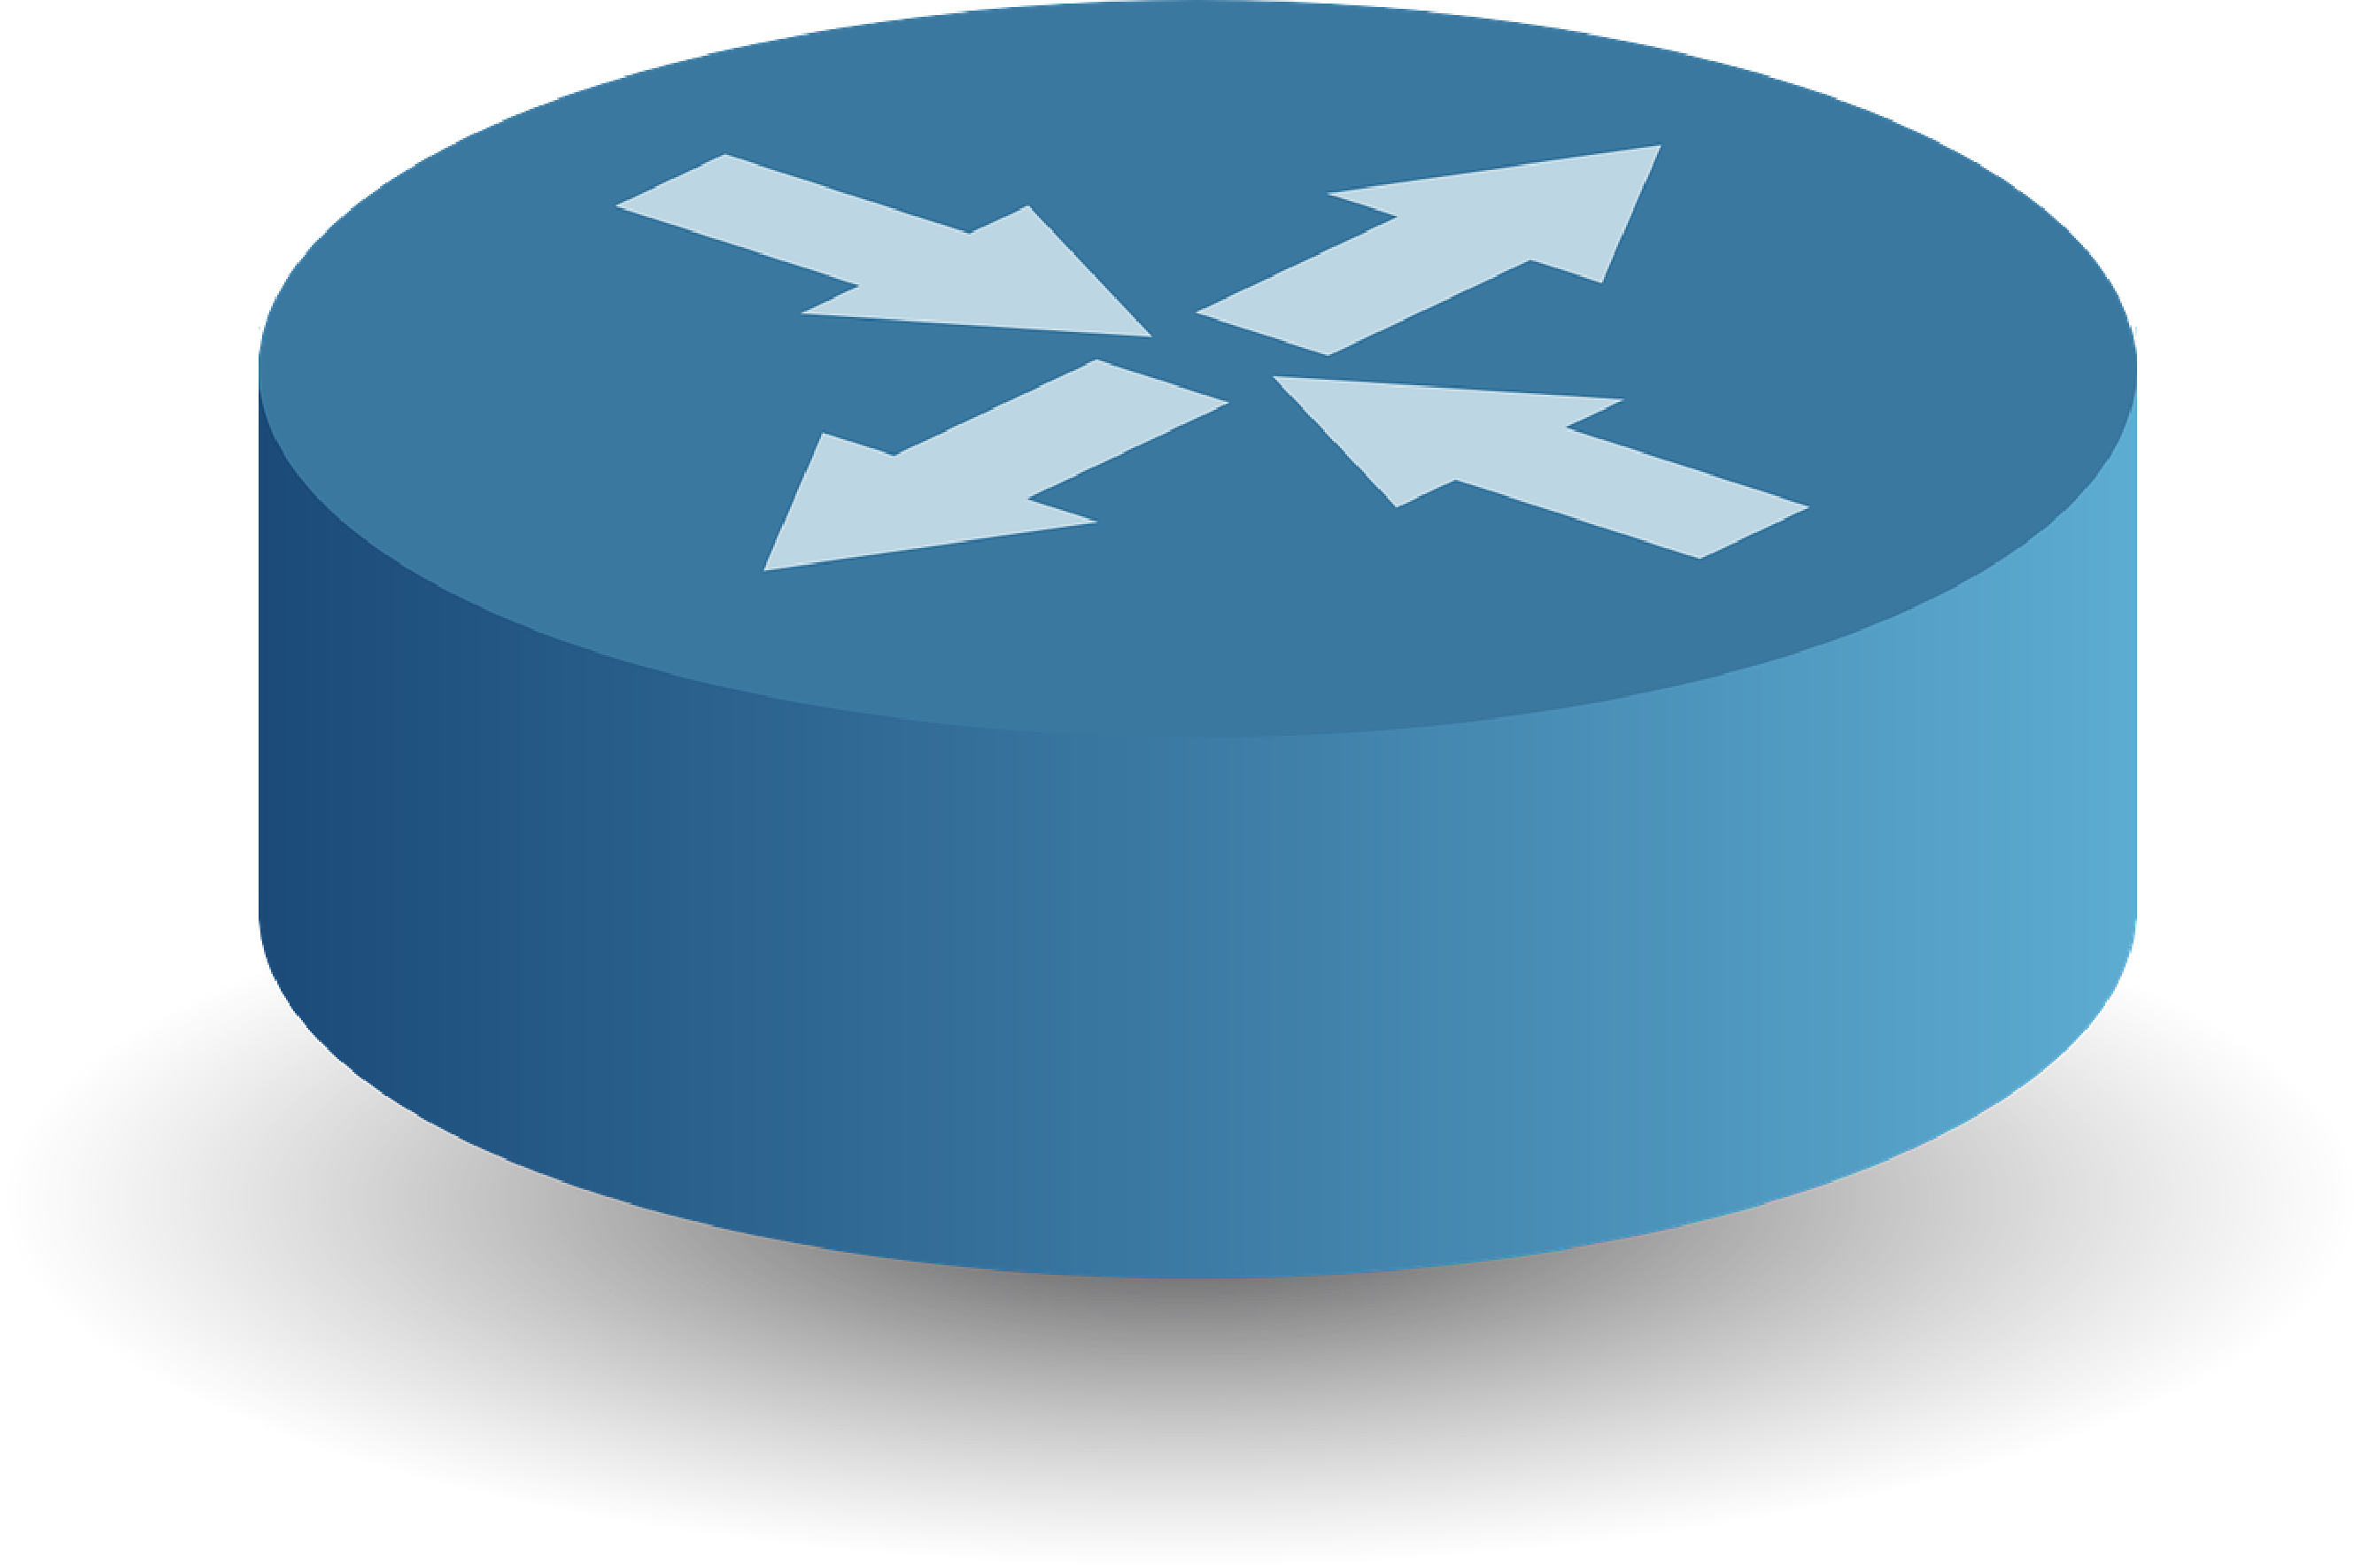
\includegraphics[width=52.5pt,height=52.5pt]{figures/router-29825_1280.pdf}};




%Rounded Rect [id:dp3362169615585995] 
\draw  [fill={rgb, 255:red, 246; green, 185; blue, 255 }  ,fill opacity=1 ] (14.33,161.8) .. controls (14.33,142.3) and (30.14,126.5) .. (49.63,126.5) -- (421.03,126.5) .. controls (440.53,126.5) and (456.33,142.3) .. (456.33,161.8) -- (456.33,267.7) .. controls (456.33,287.2) and (440.53,303) .. (421.03,303) -- (49.63,303) .. controls (30.14,303) and (14.33,287.2) .. (14.33,267.7) -- cycle ;
%Rounded Rect [id:dp9567502407138185] 
\draw  [fill={rgb, 255:red, 255; green, 255; blue, 255 }  ,fill opacity=1 ][line width=1.5]  (210.83,194.22) .. controls (210.83,190.83) and (213.58,188.08) .. (216.97,188.08) -- (310.7,188.08) .. controls (314.09,188.08) and (316.83,190.83) .. (316.83,194.22) -- (316.83,212.62) .. controls (316.83,216) and (314.09,218.75) .. (310.7,218.75) -- (216.97,218.75) .. controls (213.58,218.75) and (210.83,216) .. (210.83,212.62) -- cycle ;

%Rounded Rect [id:dp009214837373342832] 
\draw  [fill={rgb, 255:red, 255; green, 255; blue, 255 }  ,fill opacity=1 ][line width=1.5]  (51.46,194.22) .. controls (51.46,190.83) and (54.2,188.08) .. (57.59,188.08) -- (175.07,188.08) .. controls (178.46,188.08) and (181.21,190.83) .. (181.21,194.22) -- (181.21,212.62) .. controls (181.21,216) and (178.46,218.75) .. (175.07,218.75) -- (57.59,218.75) .. controls (54.2,218.75) and (51.46,216) .. (51.46,212.62) -- cycle ;

%Rounded Rect [id:dp7376385480360085] 
\draw  [fill={rgb, 255:red, 255; green, 255; blue, 255 }  ,fill opacity=1 ][line width=1.5]  (172.05,116.22) .. controls (172.05,112.83) and (174.79,110.08) .. (178.18,110.08) -- (349.49,110.08) .. controls (352.87,110.08) and (355.62,112.83) .. (355.62,116.22) -- (355.62,134.62) .. controls (355.62,138) and (352.87,140.75) .. (349.49,140.75) -- (178.18,140.75) .. controls (174.79,140.75) and (172.05,138) .. (172.05,134.62) -- cycle ;

%Rounded Rect [id:dp19791531901769066] 
\draw  [fill={rgb, 255:red, 255; green, 255; blue, 255 }  ,fill opacity=1 ][line width=1.5]  (172.05,294.22) .. controls (172.05,290.83) and (174.79,288.08) .. (178.18,288.08) -- (349.49,288.08) .. controls (352.87,288.08) and (355.62,290.83) .. (355.62,294.22) -- (355.62,312.62) .. controls (355.62,316) and (352.87,318.75) .. (349.49,318.75) -- (178.18,318.75) .. controls (174.79,318.75) and (172.05,316) .. (172.05,312.62) -- cycle ;

%Straight Lines [id:da3071607162532064] 
\draw  [dash pattern={on 4.5pt off 4.5pt}]  (262.56,144.33) -- (263.44,184.83) ;
\draw [shift={(263.5,187.83)}, rotate = 268.77] [fill={rgb, 255:red, 0; green, 0; blue, 0 }  ][line width=0.08]  [draw opacity=0] (10.72,-5.15) -- (0,0) -- (10.72,5.15) -- (7.12,0) -- cycle    ;
\draw [shift={(262.5,141.33)}, rotate = 88.77] [fill={rgb, 255:red, 0; green, 0; blue, 0 }  ][line width=0.08]  [draw opacity=0] (10.72,-5.15) -- (0,0) -- (10.72,5.15) -- (7.12,0) -- cycle    ;
%Straight Lines [id:da5811563165265446] 
\draw  [dash pattern={on 4.5pt off 4.5pt}]  (120.06,239.8) -- (119.14,220.83) ;
\draw [shift={(119,217.83)}, rotate = 447.25] [fill={rgb, 255:red, 0; green, 0; blue, 0 }  ][line width=0.08]  [draw opacity=0] (10.72,-5.15) -- (0,0) -- (10.72,5.15) -- (7.12,0) -- cycle    ;
\draw [shift={(120.2,242.8)}, rotate = 267.25] [fill={rgb, 255:red, 0; green, 0; blue, 0 }  ][line width=0.08]  [draw opacity=0] (10.72,-5.15) -- (0,0) -- (10.72,5.15) -- (7.12,0) -- cycle    ;
%Straight Lines [id:da36813314079504633] 
\draw  [dash pattern={on 4.5pt off 4.5pt}]  (189,250) -- (209.32,215.21) ;
\draw [shift={(210.83,212.62)}, rotate = 480.29] [fill={rgb, 255:red, 0; green, 0; blue, 0 }  ][line width=0.08]  [draw opacity=0] (10.72,-5.15) -- (0,0) -- (10.72,5.15) -- (7.12,0) -- cycle    ;

%Straight Lines [id:da7736079542900215] 
\draw  [dash pattern={on 4.5pt off 4.5pt}]  (263,222.83) -- (263,284.83) ;
\draw [shift={(263,287.83)}, rotate = 270] [fill={rgb, 255:red, 0; green, 0; blue, 0 }  ][line width=0.08]  [draw opacity=0] (10.72,-5.15) -- (0,0) -- (10.72,5.15) -- (7.12,0) -- cycle    ;
\draw [shift={(263,219.83)}, rotate = 90] [fill={rgb, 255:red, 0; green, 0; blue, 0 }  ][line width=0.08]  [draw opacity=0] (10.72,-5.15) -- (0,0) -- (10.72,5.15) -- (7.12,0) -- cycle    ;
%Straight Lines [id:da5692634255089728] 
\draw  [dash pattern={on 4.5pt off 4.5pt}]  (185,204.23) -- (207,203.44) ;
\draw [shift={(210,203.33)}, rotate = 537.95] [fill={rgb, 255:red, 0; green, 0; blue, 0 }  ][line width=0.08]  [draw opacity=0] (10.72,-5.15) -- (0,0) -- (10.72,5.15) -- (7.12,0) -- cycle    ;
\draw [shift={(182,204.33)}, rotate = 357.95] [fill={rgb, 255:red, 0; green, 0; blue, 0 }  ][line width=0.08]  [draw opacity=0] (10.72,-5.15) -- (0,0) -- (10.72,5.15) -- (7.12,0) -- cycle    ;
%Straight Lines [id:da11917773489604144] 
\draw  [dash pattern={on 4.5pt off 4.5pt}]  (195.8,259.02) -- (328.77,256.62) ;
\draw [shift={(331.77,256.57)}, rotate = 538.97] [fill={rgb, 255:red, 0; green, 0; blue, 0 }  ][line width=0.08]  [draw opacity=0] (10.72,-5.15) -- (0,0) -- (10.72,5.15) -- (7.12,0) -- cycle    ;

%Straight Lines [id:da7770404819607903] 
\draw  [dash pattern={on 4.5pt off 4.5pt}]  (262.81,322.31) -- (262.98,351.33) ;
\draw [shift={(263,354.33)}, rotate = 269.65999999999997] [fill={rgb, 255:red, 0; green, 0; blue, 0 }  ][line width=0.08]  [draw opacity=0] (10.72,-5.15) -- (0,0) -- (10.72,5.15) -- (7.12,0) -- cycle    ;
\draw [shift={(262.79,319.31)}, rotate = 89.66] [fill={rgb, 255:red, 0; green, 0; blue, 0 }  ][line width=0.08]  [draw opacity=0] (10.72,-5.15) -- (0,0) -- (10.72,5.15) -- (7.12,0) -- cycle    ;
%Straight Lines [id:da8379163771385384] 
\draw  [dash pattern={on 4.5pt off 4.5pt}]  (145.98,273.33) -- (145.46,349.78) ;
\draw [shift={(145.44,352.78)}, rotate = 270.39] [fill={rgb, 255:red, 0; green, 0; blue, 0 }  ][line width=0.08]  [draw opacity=0] (10.72,-5.15) -- (0,0) -- (10.72,5.15) -- (7.12,0) -- cycle    ;
\draw [shift={(146,270.33)}, rotate = 90.39] [fill={rgb, 255:red, 0; green, 0; blue, 0 }  ][line width=0.08]  [draw opacity=0] (10.72,-5.15) -- (0,0) -- (10.72,5.15) -- (7.12,0) -- cycle    ;
%Straight Lines [id:da7179548819350594] 
\draw  [dash pattern={on 4.5pt off 4.5pt}]  (263,72.33) -- (263,106.33) ;
\draw [shift={(263,109.33)}, rotate = 270] [fill={rgb, 255:red, 0; green, 0; blue, 0 }  ][line width=0.08]  [draw opacity=0] (10.72,-5.15) -- (0,0) -- (10.72,5.15) -- (7.12,0) -- cycle    ;
\draw [shift={(263,69.33)}, rotate = 90] [fill={rgb, 255:red, 0; green, 0; blue, 0 }  ][line width=0.08]  [draw opacity=0] (10.72,-5.15) -- (0,0) -- (10.72,5.15) -- (7.12,0) -- cycle    ;
%Rounded Rect [id:dp3518984914276363] 
\draw  [fill={rgb, 255:red, 56; green, 144; blue, 249 }  ,fill opacity=1 ] (121.5,17.37) .. controls (121.5,9.98) and (127.48,4) .. (134.87,4) -- (361.13,4) .. controls (368.52,4) and (374.5,9.98) .. (374.5,17.37) -- (374.5,57.47) .. controls (374.5,64.85) and (368.52,70.83) .. (361.13,70.83) -- (134.87,70.83) .. controls (127.48,70.83) and (121.5,64.85) .. (121.5,57.47) -- cycle ;
%Rounded Rect [id:dp09188382569915587] 
\draw  [color={rgb, 255:red, 0; green, 0; blue, 0 }  ,draw opacity=1 ][fill={rgb, 255:red, 255; green, 255; blue, 255 }  ,fill opacity=1 ][dash pattern={on 5.63pt off 4.5pt}][line width=1.5]  (129.7,35.2) .. controls (129.7,31.87) and (132.4,29.17) .. (135.73,29.17) -- (234.94,29.17) .. controls (238.27,29.17) and (240.97,31.87) .. (240.97,35.2) -- (240.97,53.3) .. controls (240.97,56.63) and (238.27,59.33) .. (234.94,59.33) -- (135.73,59.33) .. controls (132.4,59.33) and (129.7,56.63) .. (129.7,53.3) -- cycle ;
%Rounded Rect [id:dp24603064281963627] 
\draw  [color={rgb, 255:red, 0; green, 0; blue, 0 }  ,draw opacity=1 ][fill={rgb, 255:red, 255; green, 255; blue, 255 }  ,fill opacity=1 ][dash pattern={on 5.63pt off 4.5pt}][line width=1.5]  (255.03,35.2) .. controls (255.03,31.87) and (257.73,29.17) .. (261.06,29.17) -- (360.27,29.17) .. controls (363.6,29.17) and (366.3,31.87) .. (366.3,35.2) -- (366.3,53.3) .. controls (366.3,56.63) and (363.6,59.33) .. (360.27,59.33) -- (261.06,59.33) .. controls (257.73,59.33) and (255.03,56.63) .. (255.03,53.3) -- cycle ;

%Rounded Rect [id:dp758697930562836] 
\draw  [fill={rgb, 255:red, 255; green, 255; blue, 255 }  ,fill opacity=1 ][line width=1.5]  (109.06,245.55) .. controls (109.06,242.16) and (111.81,239.42) .. (115.19,239.42) -- (191.47,239.42) .. controls (194.86,239.42) and (197.6,242.16) .. (197.6,245.55) -- (197.6,263.95) .. controls (197.6,267.34) and (194.86,270.08) .. (191.47,270.08) -- (115.19,270.08) .. controls (111.81,270.08) and (109.06,267.34) .. (109.06,263.95) -- cycle ;

%Straight Lines [id:da6795518551939627] 
\draw  [dash pattern={on 4.5pt off 4.5pt}]  (325,143.83) -- (324.78,284.78) ;
\draw [shift={(324.78,287.78)}, rotate = 270.09000000000003] [fill={rgb, 255:red, 0; green, 0; blue, 0 }  ][line width=0.08]  [draw opacity=0] (10.72,-5.15) -- (0,0) -- (10.72,5.15) -- (7.12,0) -- cycle    ;
\draw [shift={(325,140.83)}, rotate = 90.09] [fill={rgb, 255:red, 0; green, 0; blue, 0 }  ][line width=0.08]  [draw opacity=0] (10.72,-5.15) -- (0,0) -- (10.72,5.15) -- (7.12,0) -- cycle    ;
%Straight Lines [id:da055910518428688105] 
\draw  [dash pattern={on 4.5pt off 4.5pt}]  (185.78,140.44) -- (185.72,236.92) ;
\draw [shift={(185.72,239.92)}, rotate = 270.03] [fill={rgb, 255:red, 0; green, 0; blue, 0 }  ][line width=0.08]  [draw opacity=0] (10.72,-5.15) -- (0,0) -- (10.72,5.15) -- (7.12,0) -- cycle    ;

%Straight Lines [id:da9613526114203358] 
\draw  [dash pattern={on 4.5pt off 4.5pt}]  (66.42,221.44) -- (65.78,295.78) -- (169.05,294.26) ;
\draw [shift={(172.05,294.22)}, rotate = 539.1600000000001] [fill={rgb, 255:red, 0; green, 0; blue, 0 }  ][line width=0.08]  [draw opacity=0] (10.72,-5.15) -- (0,0) -- (10.72,5.15) -- (7.12,0) -- cycle    ;
\draw [shift={(66.44,218.44)}, rotate = 90.49] [fill={rgb, 255:red, 0; green, 0; blue, 0 }  ][line width=0.08]  [draw opacity=0] (10.72,-5.15) -- (0,0) -- (10.72,5.15) -- (7.12,0) -- cycle    ;
%Straight Lines [id:da3742893196331808] 
\draw  [dash pattern={on 4.5pt off 4.5pt}]  (348.07,143.83) -- (350.1,234.17) ;
\draw [shift={(350.17,237.17)}, rotate = 268.71] [fill={rgb, 255:red, 0; green, 0; blue, 0 }  ][line width=0.08]  [draw opacity=0] (10.72,-5.15) -- (0,0) -- (10.72,5.15) -- (7.12,0) -- cycle    ;
\draw [shift={(348,140.83)}, rotate = 88.71] [fill={rgb, 255:red, 0; green, 0; blue, 0 }  ][line width=0.08]  [draw opacity=0] (10.72,-5.15) -- (0,0) -- (10.72,5.15) -- (7.12,0) -- cycle    ;
%Rounded Rect [id:dp9140860086605985] 
\draw  [fill={rgb, 255:red, 255; green, 255; blue, 255 }  ,fill opacity=1 ][line width=1.5]  (335.83,245.55) .. controls (335.83,242.16) and (338.58,239.42) .. (341.97,239.42) -- (435.7,239.42) .. controls (439.09,239.42) and (441.83,242.16) .. (441.83,245.55) -- (441.83,263.95) .. controls (441.83,267.34) and (439.09,270.08) .. (435.7,270.08) -- (341.97,270.08) .. controls (338.58,270.08) and (335.83,267.34) .. (335.83,263.95) -- cycle ;

%Shape: Ellipse [id:dp3554083551130477] 
\draw  [color={rgb, 255:red, 208; green, 2; blue, 27 }  ,draw opacity=1 ] (188.3,153.75) .. controls (188.3,149.91) and (191.71,146.8) .. (195.93,146.8) .. controls (200.14,146.8) and (203.55,149.91) .. (203.55,153.75) .. controls (203.55,157.59) and (200.14,160.7) .. (195.93,160.7) .. controls (191.71,160.7) and (188.3,157.59) .. (188.3,153.75) -- cycle ;
%Shape: Ellipse [id:dp4084549692042517] 
\draw  [color={rgb, 255:red, 208; green, 2; blue, 27 }  ,draw opacity=1 ] (267.05,87.25) .. controls (267.05,83.41) and (270.46,80.3) .. (274.68,80.3) .. controls (278.89,80.3) and (282.3,83.41) .. (282.3,87.25) .. controls (282.3,91.09) and (278.89,94.2) .. (274.68,94.2) .. controls (270.46,94.2) and (267.05,91.09) .. (267.05,87.25) -- cycle ;
%Shape: Ellipse [id:dp6652927550013479] 
\draw  [color={rgb, 255:red, 208; green, 2; blue, 27 }  ,draw opacity=1 ] (264.8,156.5) .. controls (264.8,152.66) and (268.21,149.55) .. (272.43,149.55) .. controls (276.64,149.55) and (280.05,152.66) .. (280.05,156.5) .. controls (280.05,160.34) and (276.64,163.45) .. (272.43,163.45) .. controls (268.21,163.45) and (264.8,160.34) .. (264.8,156.5) -- cycle ;
%Shape: Ellipse [id:dp20966000134493123] 
\draw  [color={rgb, 255:red, 208; green, 2; blue, 27 }  ,draw opacity=1 ] (307.55,151.25) .. controls (307.55,147.41) and (310.96,144.3) .. (315.18,144.3) .. controls (319.39,144.3) and (322.8,147.41) .. (322.8,151.25) .. controls (322.8,155.09) and (319.39,158.2) .. (315.18,158.2) .. controls (310.96,158.2) and (307.55,155.09) .. (307.55,151.25) -- cycle ;
%Shape: Ellipse [id:dp0540432112177649] 
\draw  [color={rgb, 255:red, 208; green, 2; blue, 27 }  ,draw opacity=1 ] (355.55,180.75) .. controls (355.55,176.91) and (358.96,173.8) .. (363.18,173.8) .. controls (367.39,173.8) and (370.8,176.91) .. (370.8,180.75) .. controls (370.8,184.59) and (367.39,187.7) .. (363.18,187.7) .. controls (358.96,187.7) and (355.55,184.59) .. (355.55,180.75) -- cycle ;
%Shape: Ellipse [id:dp45917488569940357] 
\draw  [color={rgb, 255:red, 208; green, 2; blue, 27 }  ,draw opacity=1 ] (185.3,189.34) .. controls (185.3,185.5) and (188.71,182.39) .. (192.93,182.39) .. controls (197.14,182.39) and (200.55,185.5) .. (200.55,189.34) .. controls (200.55,193.17) and (197.14,196.28) .. (192.93,196.28) .. controls (188.71,196.28) and (185.3,193.17) .. (185.3,189.34) -- cycle ;

%Shape: Ellipse [id:dp5545246337247209] 
\draw  [color={rgb, 255:red, 208; green, 2; blue, 27 }  ,draw opacity=1 ] (199.3,229) .. controls (199.3,225.16) and (202.71,222.05) .. (206.93,222.05) .. controls (211.14,222.05) and (214.55,225.16) .. (214.55,229) .. controls (214.55,232.84) and (211.14,235.95) .. (206.93,235.95) .. controls (202.71,235.95) and (199.3,232.84) .. (199.3,229) -- cycle ;
%Shape: Ellipse [id:dp4152293630769399] 
\draw  [color={rgb, 255:red, 208; green, 2; blue, 27 }  ,draw opacity=1 ] (264.1,229.6) .. controls (264.1,225.76) and (267.51,222.65) .. (271.73,222.65) .. controls (275.94,222.65) and (279.35,225.76) .. (279.35,229.6) .. controls (279.35,233.44) and (275.94,236.55) .. (271.73,236.55) .. controls (267.51,236.55) and (264.1,233.44) .. (264.1,229.6) -- cycle ;
%Shape: Ellipse [id:dp7028700683432993] 
\draw  [color={rgb, 255:red, 208; green, 2; blue, 27 }  ,draw opacity=1 ] (230.1,249.27) .. controls (230.1,245.43) and (233.51,242.32) .. (237.73,242.32) .. controls (241.94,242.32) and (245.35,245.43) .. (245.35,249.27) .. controls (245.35,253.11) and (241.94,256.22) .. (237.73,256.22) .. controls (233.51,256.22) and (230.1,253.11) .. (230.1,249.27) -- cycle ;
%Shape: Ellipse [id:dp07410075663096749] 
\draw  [color={rgb, 255:red, 208; green, 2; blue, 27 }  ,draw opacity=1 ] (121.1,228.62) .. controls (121.1,224.05) and (125.15,220.35) .. (130.15,220.35) .. controls (135.15,220.35) and (139.2,224.05) .. (139.2,228.62) .. controls (139.2,233.18) and (135.15,236.88) .. (130.15,236.88) .. controls (125.15,236.88) and (121.1,233.18) .. (121.1,228.62) -- cycle ;
%Shape: Ellipse [id:dp30224928873301715] 
\draw  [color={rgb, 255:red, 208; green, 2; blue, 27 }  ,draw opacity=1 ] (68.3,284.22) .. controls (68.3,279.65) and (72.35,275.95) .. (77.35,275.95) .. controls (82.35,275.95) and (86.4,279.65) .. (86.4,284.22) .. controls (86.4,288.78) and (82.35,292.48) .. (77.35,292.48) .. controls (72.35,292.48) and (68.3,288.78) .. (68.3,284.22) -- cycle ;
%Shape: Ellipse [id:dp3894329820493001] 
\draw  [color={rgb, 255:red, 208; green, 2; blue, 27 }  ,draw opacity=1 ] (149.5,280.62) .. controls (149.5,276.05) and (153.55,272.35) .. (158.55,272.35) .. controls (163.55,272.35) and (167.6,276.05) .. (167.6,280.62) .. controls (167.6,285.18) and (163.55,288.88) .. (158.55,288.88) .. controls (153.55,288.88) and (149.5,285.18) .. (149.5,280.62) -- cycle ;
%Shape: Ellipse [id:dp8973642196115625] 
\draw  [color={rgb, 255:red, 208; green, 2; blue, 27 }  ,draw opacity=1 ] (375.5,281.22) .. controls (375.5,276.65) and (379.55,272.95) .. (384.55,272.95) .. controls (389.55,272.95) and (393.6,276.65) .. (393.6,281.22) .. controls (393.6,285.78) and (389.55,289.48) .. (384.55,289.48) .. controls (379.55,289.48) and (375.5,285.78) .. (375.5,281.22) -- cycle ;
%Shape: Ellipse [id:dp6431628695495194] 
\draw  [color={rgb, 255:red, 208; green, 2; blue, 27 }  ,draw opacity=1 ] (265.5,335.02) .. controls (265.5,330.45) and (269.55,326.75) .. (274.55,326.75) .. controls (279.55,326.75) and (283.6,330.45) .. (283.6,335.02) .. controls (283.6,339.58) and (279.55,343.28) .. (274.55,343.28) .. controls (269.55,343.28) and (265.5,339.58) .. (265.5,335.02) -- cycle ;
%Straight Lines [id:da6717664493405898] 
\draw  [dash pattern={on 4.5pt off 4.5pt}]  (404.17,275.17) -- (404.17,293.17) -- (355.62,294.22) ;

\draw [shift={(404.17,272.17)}, rotate = 90] [fill={rgb, 255:red, 0; green, 0; blue, 0 }  ][line width=0.08]  [draw opacity=0] (10.72,-5.15) -- (0,0) -- (10.72,5.15) -- (7.12,0) -- cycle    ;

% Text Node
\draw (106.66,137.09) node  [font=\small] [align=left] {Network Hypervisor};
% Text Node
\draw (196.26,154.45) node  [color={rgb, 255:red, 208; green, 2; blue, 27 }  ,opacity=1 ] [align=left] {3};
% Text Node
\draw (275.01,86.95) node  [color={rgb, 255:red, 208; green, 2; blue, 27 }  ,opacity=1 ] [align=left] {1};
% Text Node
\draw (272.76,157.2) node  [font=\small,color={rgb, 255:red, 208; green, 2; blue, 27 }  ,opacity=1 ] [align=left] {2};
% Text Node
\draw (314.51,151.95) node  [font=\small,color={rgb, 255:red, 208; green, 2; blue, 27 }  ,opacity=1 ] [align=left] {4};
% Text Node
\draw (364.55,180.75) node  [font=\small,color={rgb, 255:red, 208; green, 2; blue, 27 }  ,opacity=1 ] [align=left] {5};
% Text Node
\draw (207.26,228.7) node  [font=\small,color={rgb, 255:red, 208; green, 2; blue, 27 }  ,opacity=1 ] [align=left] {7};
% Text Node
\draw (272.06,229.3) node  [font=\small,color={rgb, 255:red, 208; green, 2; blue, 27 }  ,opacity=1 ] [align=left] {8};
% Text Node
\draw (238.06,248.97) node  [font=\small,color={rgb, 255:red, 208; green, 2; blue, 27 }  ,opacity=1 ] [align=left] {9};
% Text Node
\draw (130.15,228.62) node  [font=\small,color={rgb, 255:red, 208; green, 2; blue, 27 }  ,opacity=1 ] [align=left] {{\small 10}};
% Text Node
\draw (77.35,284.22) node  [color={rgb, 255:red, 208; green, 2; blue, 27 }  ,opacity=1 ] [align=left] {{\small 11}};
% Text Node
\draw (157.55,280.62) node  [font=\small,color={rgb, 255:red, 208; green, 2; blue, 27 }  ,opacity=1 ] [align=left] {{\small 12}};
% Text Node
\draw (383.55,279.22) node  [color={rgb, 255:red, 208; green, 2; blue, 27 }  ,opacity=1 ] [align=left] {{\small 13}};
% Text Node
\draw (274.15,334.62) node  [color={rgb, 255:red, 208; green, 2; blue, 27 }  ,opacity=1 ] [align=left] {{\small 14}};
% Text Node
\draw (192.76,189.03) node  [color={rgb, 255:red, 208; green, 2; blue, 27 }  ,opacity=1 ] [align=left] {6};
% Text Node
\draw (388.83,256.08) node   [align=left] {Security};
% Text Node
\draw (153.33,256.08) node   [align=left] {Monitoring};
% Text Node
\draw (160.93,11.75) node  [font=\small,color={rgb, 255:red, 0; green, 0; blue, 0 }  ,opacity=1 ] [align=left] {Tenants};
% Text Node
\draw (310.08,45.17) node   [align=left] {\textcolor[rgb]{0,0,0}{Controllers}};
% Text Node
\draw (184.75,45.17) node   [align=left] {\textcolor[rgb]{0,0,0}{Applications}};
% Text Node
\draw (263.83,304.75) node   [align=left] {Data Plane Abstraction};
% Text Node
\draw (263.83,126.75) node   [align=left] {Control Plane Abstraction};
% Text Node
\draw (116.33,204.75) node   [align=left] {Resource Isolator};
% Text Node
\draw (263.83,204.75) node   [align=left] {VN Embedding};
% Text Node
\draw (143.66,363.17) node  [font=\small] [align=left] {Physical Infrastructure};


\end{tikzpicture}

\caption{Reference architecture of a network hypervisor}
\label{fig:reference-archi-nh}
\end{figure}
  
Figure~\ref{fig:reference-archi-nh} presents the the reference architecture of a network hypervisor.
On a top-down perspective, there are three different levels in the reference architecture.
The tenant level, where end-users can deploy their own applications, SDN controllers, etc.
The hypervisor level, including all the components required to achieve network virtualization and present the tenant with an abstract view.
The lowest level includes all the networking equipments, like SDN-enabled switches and routers.

\paragraph{Control Plane Abstraction}
The Control Plane Abstraction component (CPAC) provides the tenants with an interface to interact with the rest of the virtualization layer.
This component is essential to the functioning of a network hypervisor and is implemented in every hypervisor.
When a tenant requests a virtual topology, he describes his requirements in terms of virtual nodes, links, minimal bandwidth, security etc. This request is received by the CPAC that will transmit it to the VN Embedding component for further treatment.
CPAC also defines tenants' capacities to interact with their virtual network, which can be either hypervisor based control or full control.
Hypervisor based control limits the capacities of the tenants by only exposing an API to interact with their slice in a specific manner. For instance, the tenant may only use the API of the hypervisor or must use a specific programming language to implement his applications for the hypervisor~\cite{FlowN-Drutskoy2012,NetworkHypervisor-Huang2013}. 
The full control describes an hypervisor where the tenant can use any application or SDN controller to interact with his virtual network. The tenant is not constrained by technical limitations of the hypervisor's components.
This is achieved by exposing a standard interface to the tenant (\eg OpenFlow~\cite{Openflow-McKeown2008}).


\paragraph{Data Plane Abstraction}
\label{sec:abstraction_comp}
The Data Plane Abstraction Component (DPAC) abstracts the physical infrastructure to serve each tenant with their own topology and resources.
Similarly to the CPAC, this component is essential and implemented in every hypervisor.
It maintains the mapping between logical and physical topology to translate logical decisions into physical one.
It also makes sure the interactions of a tenant with its virtual network does not compromise the operations of other tenants. When a tenant deploys a new configuration in his network, like routing protocols, ACLs etc., the DPAC is in charge of translating the virtual parameters and values used by the tenant into the corresponding ones for the physical infrastructure.

In practice, the abstraction can be done for several resources:

\subparagraph{\textbf{Topology}}\textbf{}\\
The hypervisor decouples the logical topology required by the tenant from the physical infrastructure.
Topology mapping can be either 1-to-1 or many-to-1. 
The first mapping corresponds to the case where one virtual node is embedded on one physical node, similarly FlowVisor~\cite{FlowVisor-Sherwood2009} where the physical infrastructure is sliced and a small portion of it is presented to each tenant.
The second one abstracts several physical nodes and links to a virtual single node or link, as  presented in~\cite{OpenVirteX-Al-Shabibi2014}.
A particular approach is when the tenants only requires one virtual node to interconnect his VMs, and does not want to bear the burden of maintaining physical equipments, or the enforce routing etc. This approach is referred in the literature as the ``Big Switch Abstraction".


\subparagraph{\textbf{Flowspace}}\textbf{}\\
The flowspace of a virtual network defines the range of values in the header fields a tenant can use in his addressing and routing schemes or if he can exploit the whole address range and other header fields.
This includes MAC addresses, IP addresses, transport layer ports, VLAN ID etc.
FlowVisor~\cite{FlowVisor-Sherwood2009} requires to share the flowspace among all tenants while other solutions like OpenVirteX~\cite{OpenVirteX-Al-Shabibi2014} offer a full address space virtualization.

\subparagraph{\textbf{Node Resources}}\textbf{}\\
The resources provided by a physical node are CPU power, and flow tables entries.
These resources are dissociated because they serve two distinct goals.
CPU provides computation power for incoming packets and defines the forwarding capacity.
Flow tables store the rules each tenant had inserted in the node.
Therefore one tenant can have high CPU percentage with a small flow table if the point is to switch multiple packets to a small set of sources and destination.

\subparagraph{\textbf{Link Resources}}\textbf{}\\
We consider here the bandwidth and the buffer
Abstracting the physical link resources is done by giving access to the bandwidth and the links' buffers to the tenants.
As presented for the node resources, link resources can be shared independently.
Depending on the usage of the resources desired by each tenant, one might big buffers for reception but a low bandwidth to transmit the packets.
Another only requires a minimum bandwidth on each virtual link.

\begin{figure}[ht]
\centering



\tikzset{every picture/.style={line width=0.75pt}} %set default line width to 0.75pt        

\scalebox{0.7}{\begin{tikzpicture}[x=0.75pt,y=0.75pt,yscale=-1,xscale=1]
%uncomment if require: \path (0,434.5); %set diagram left start at 0, and has height of 434.5

%Rounded Rect [id:dp5238736497415925] 
\draw  [fill={rgb, 255:red, 242; green, 175; blue, 175 }  ,fill opacity=1 ] (292,78.23) .. controls (292,67.98) and (300.31,59.67) .. (310.57,59.67) -- (524.43,59.67) .. controls (534.69,59.67) and (543,67.98) .. (543,78.23) -- (543,133.93) .. controls (543,144.19) and (534.69,152.5) .. (524.43,152.5) -- (310.57,152.5) .. controls (300.31,152.5) and (292,144.19) .. (292,133.93) -- cycle ;
%Straight Lines [id:da8274436550735994] 
\draw    (336,121.5) -- (497,116.67) ;


%Image [id:dp7319392175317063] 
\draw (327,120.5) node  {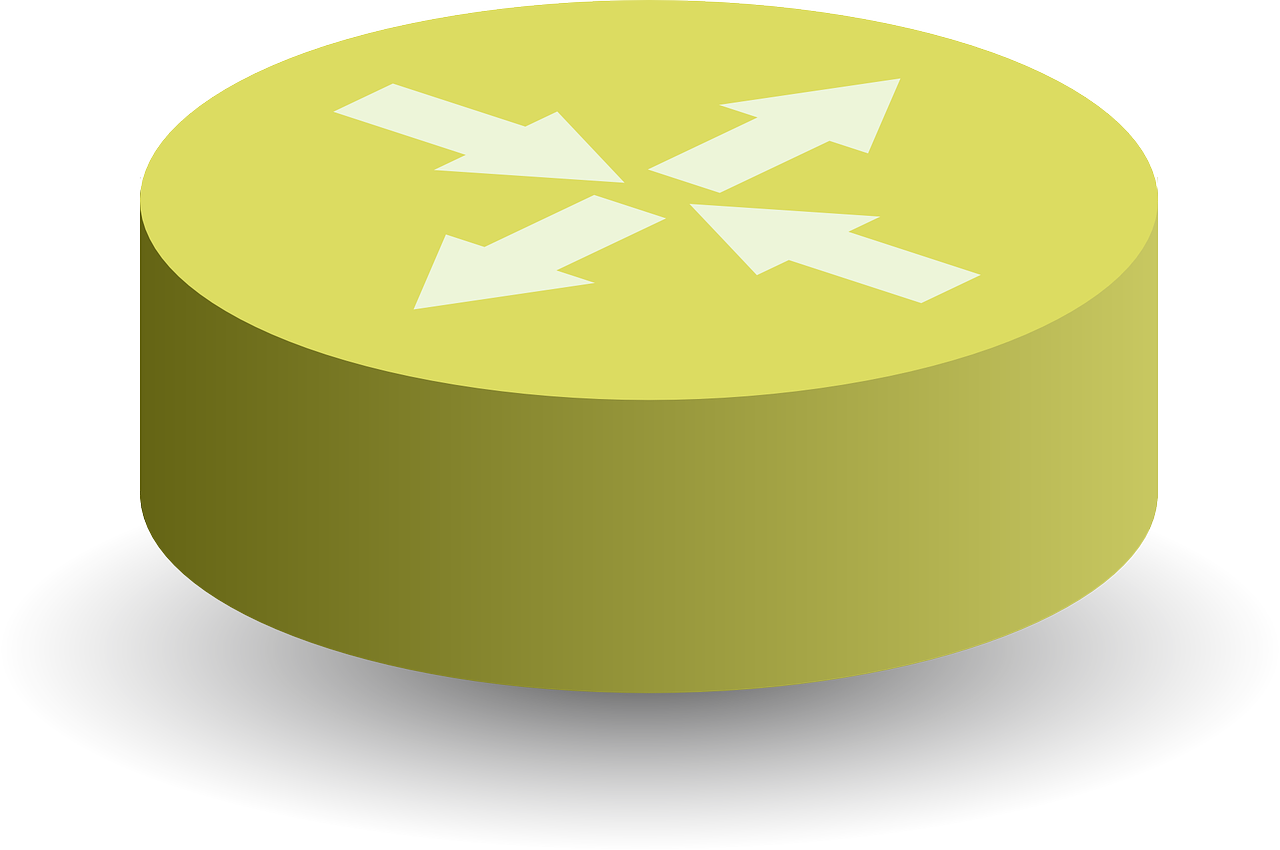
\includegraphics[width=52.5pt,height=52.5pt]{figures/router-158644_1280.png}};
%Image [id:dp370061399936939] 
\draw (412.5,120.5) node  {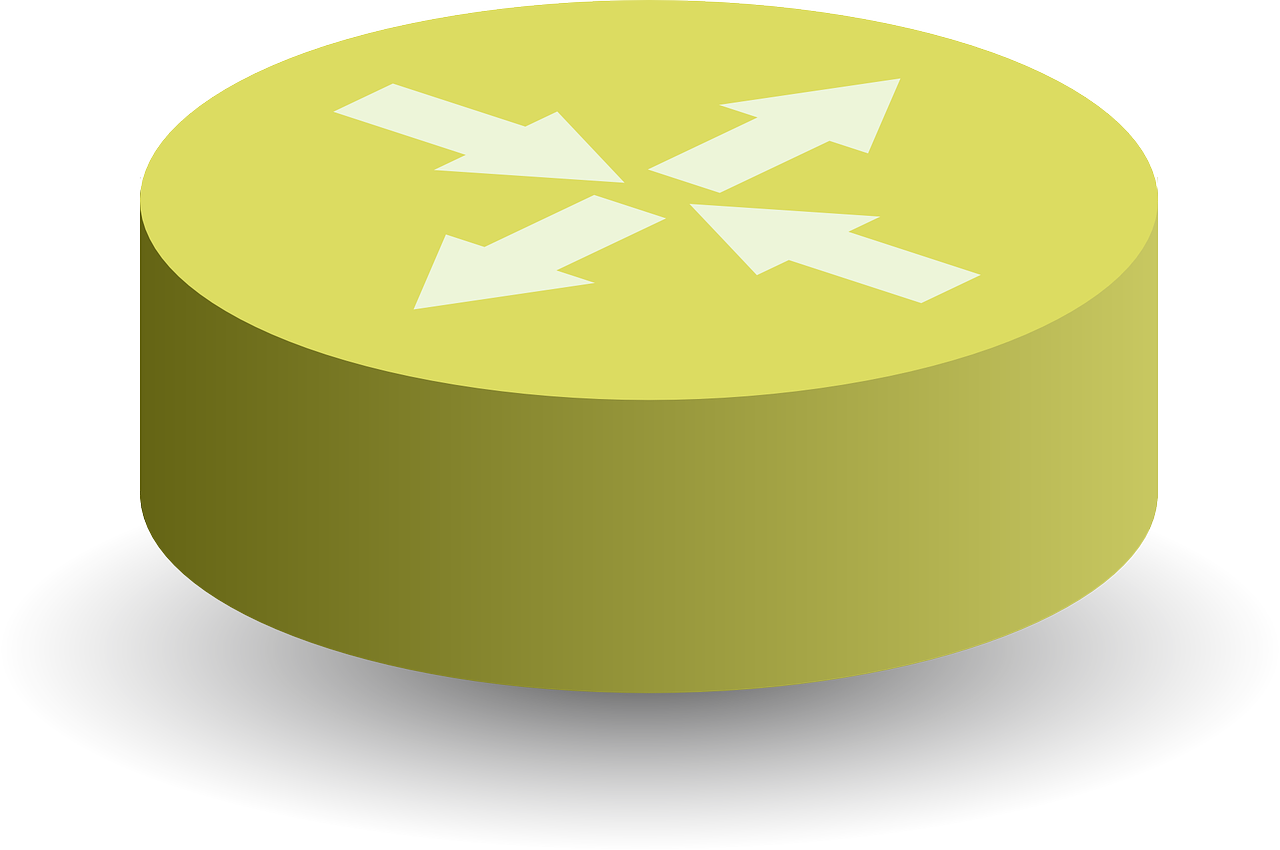
\includegraphics[width=52.5pt,height=52.5pt]{figures/router-158644_1280.png}};
%Image [id:dp4531875445870204] 
\draw (502,120.5) node  {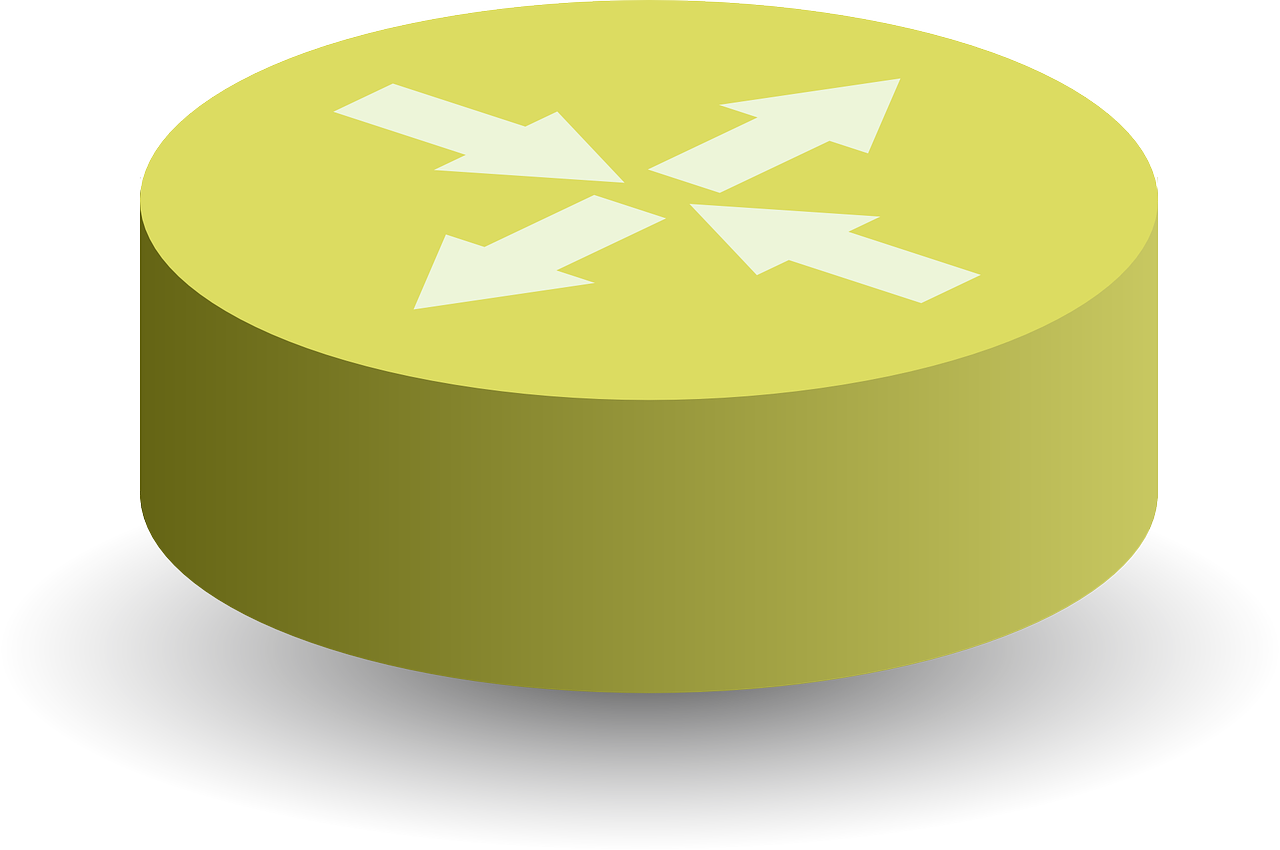
\includegraphics[width=52.5pt,height=52.5pt]{figures/router-158644_1280.png}};

%Rounded Rect [id:dp47820441471440045] 
\draw  [fill={rgb, 255:red, 255; green, 248; blue, 177 }  ,fill opacity=1 ] (46,95.27) .. controls (46,75.05) and (62.39,58.67) .. (82.6,58.67) -- (198.4,58.67) .. controls (218.61,58.67) and (235,75.05) .. (235,95.27) -- (235,205.07) .. controls (235,225.28) and (218.61,241.67) .. (198.4,241.67) -- (82.6,241.67) .. controls (62.39,241.67) and (46,225.28) .. (46,205.07) -- cycle ;
%Straight Lines [id:da6763053778165418] 
\draw    (76,150.67) -- (186,104.67) ;


%Image [id:dp8140812900187272] 
\draw (81,154.5) node  {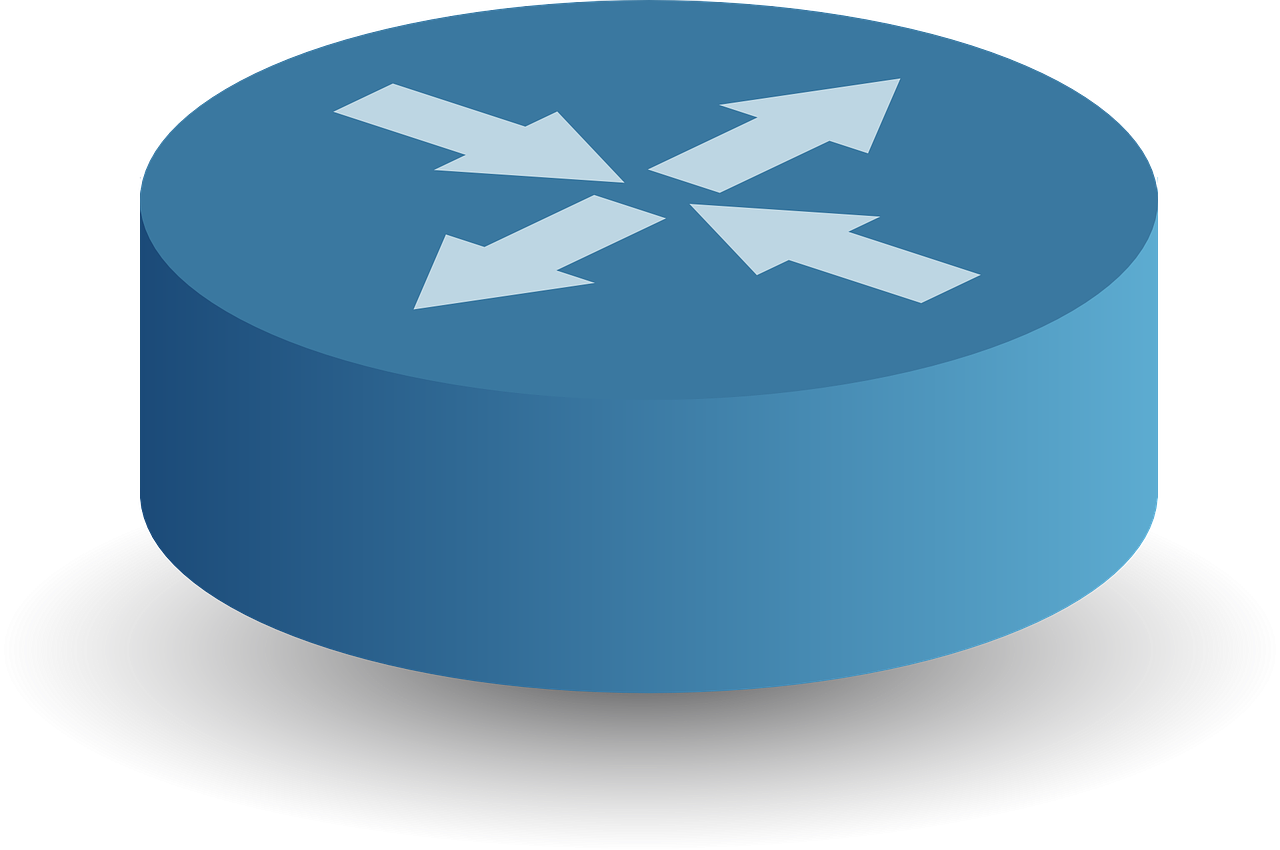
\includegraphics[width=52.5pt,height=52.5pt]{figures/router-29825_1280.png}};
%Image [id:dp7802067738931798] 
\draw (185,100.5) node  {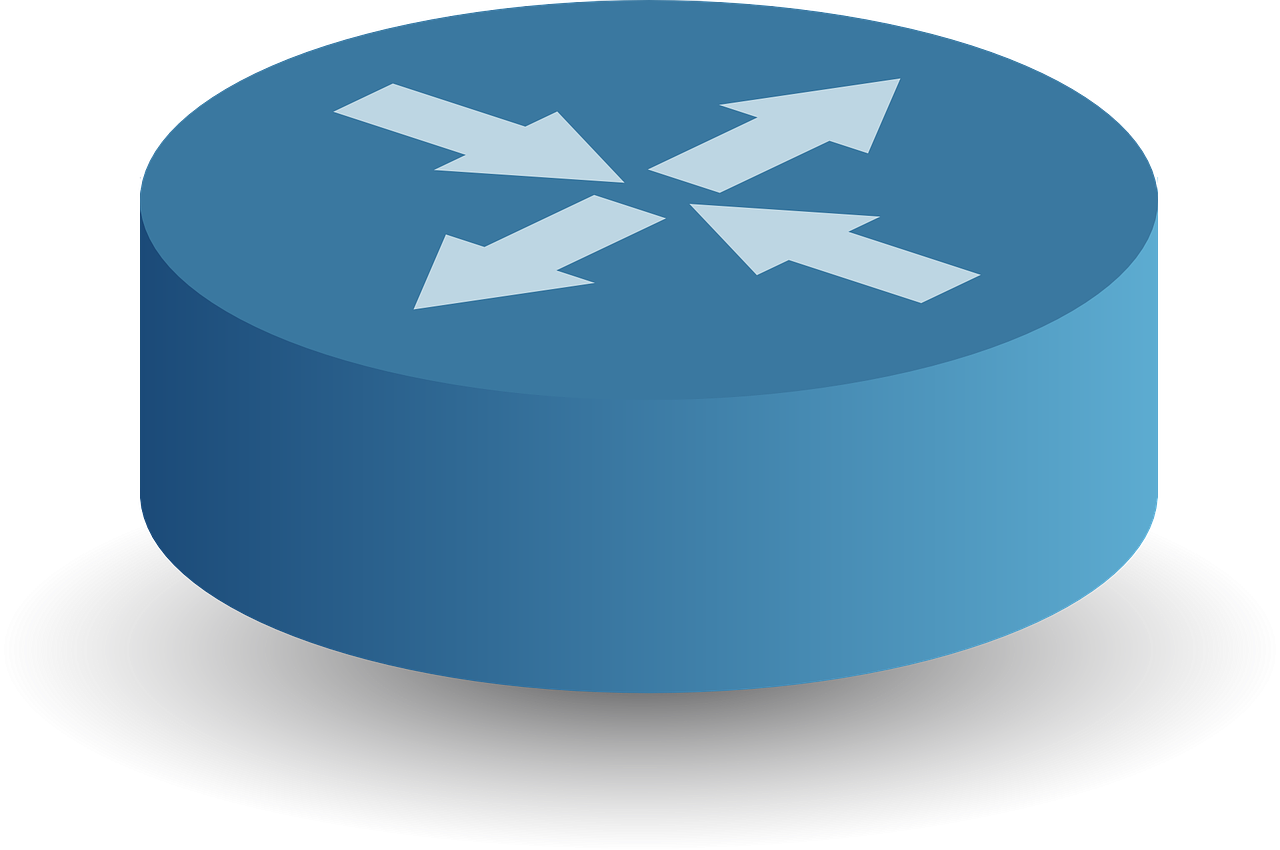
\includegraphics[width=52.5pt,height=52.5pt]{figures/router-29825_1280.png}};

%Straight Lines [id:da4951165105339822] 
\draw    (101,170.17) -- (158,195.67) ;


%Image [id:dp7416941722348419] 
\draw (156,208.5) node  {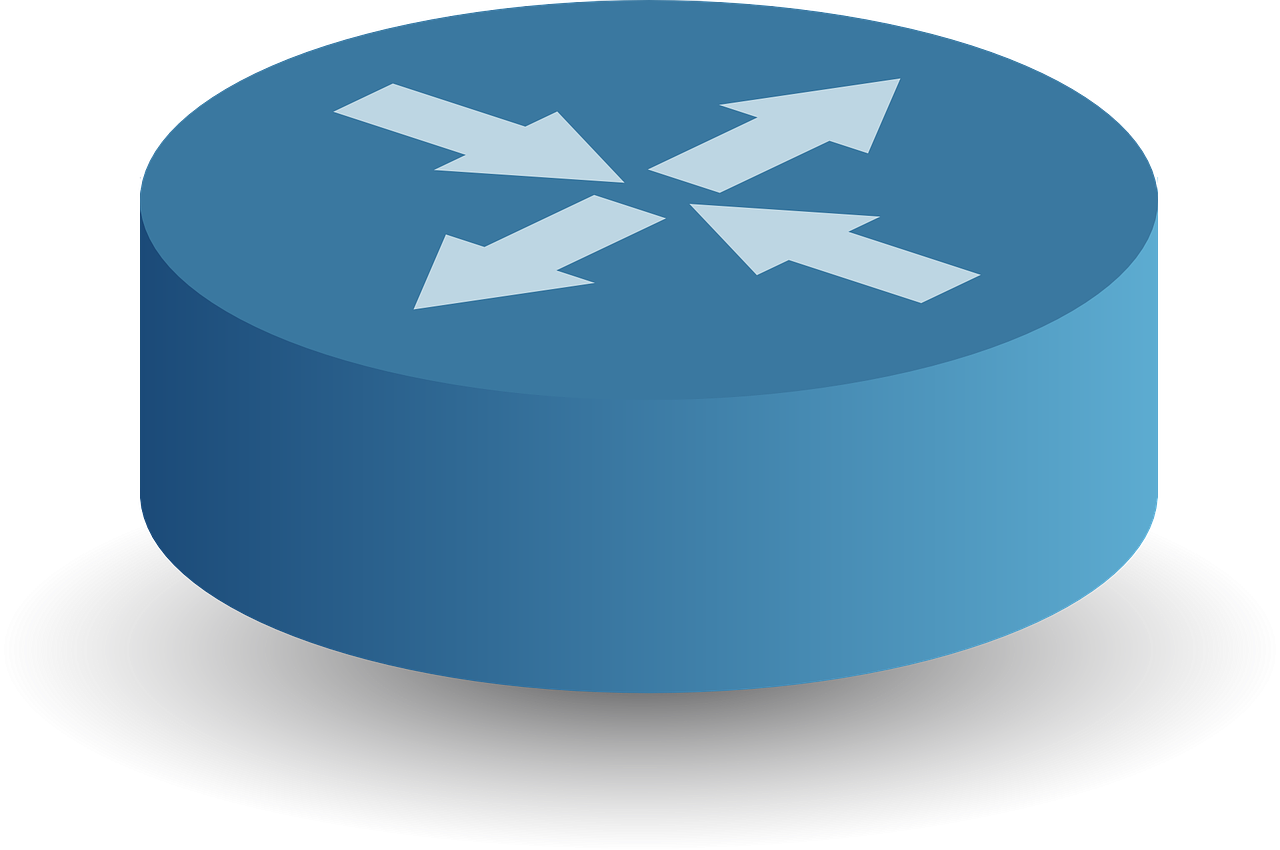
\includegraphics[width=52.5pt,height=52.5pt]{figures/router-29825_1280.png}};

%Rounded Rect [id:dp24159584532295242] 
\draw  [fill={rgb, 255:red, 184; green, 233; blue, 134 }  ,fill opacity=1 ] (27,297.47) .. controls (27,282.11) and (39.45,269.67) .. (54.8,269.67) -- (602.2,269.67) .. controls (617.55,269.67) and (630,282.11) .. (630,297.47) -- (630,380.87) .. controls (630,396.22) and (617.55,408.67) .. (602.2,408.67) -- (54.8,408.67) .. controls (39.45,408.67) and (27,396.22) .. (27,380.87) -- cycle ;
%Straight Lines [id:da4431598038778879] 
\draw    (99,327.67) -- (234,300.67) ;


%Straight Lines [id:da13869241806959443] 
\draw    (100,342.67) -- (191,365.67) ;


%Straight Lines [id:da638319369024069] 
\draw    (194,372.67) -- (388,325.67) ;


%Straight Lines [id:da0876024287705166] 
\draw    (234,300.67) -- (378,309.67) ;


%Straight Lines [id:da03053485372734699] 
\draw    (404,319.67) -- (522,306.67) ;


%Straight Lines [id:da8278064324522899] 
\draw    (395,339.67) -- (497,375.67) ;


%Image [id:dp619468693007916] 
\draw (90,342.5) node  {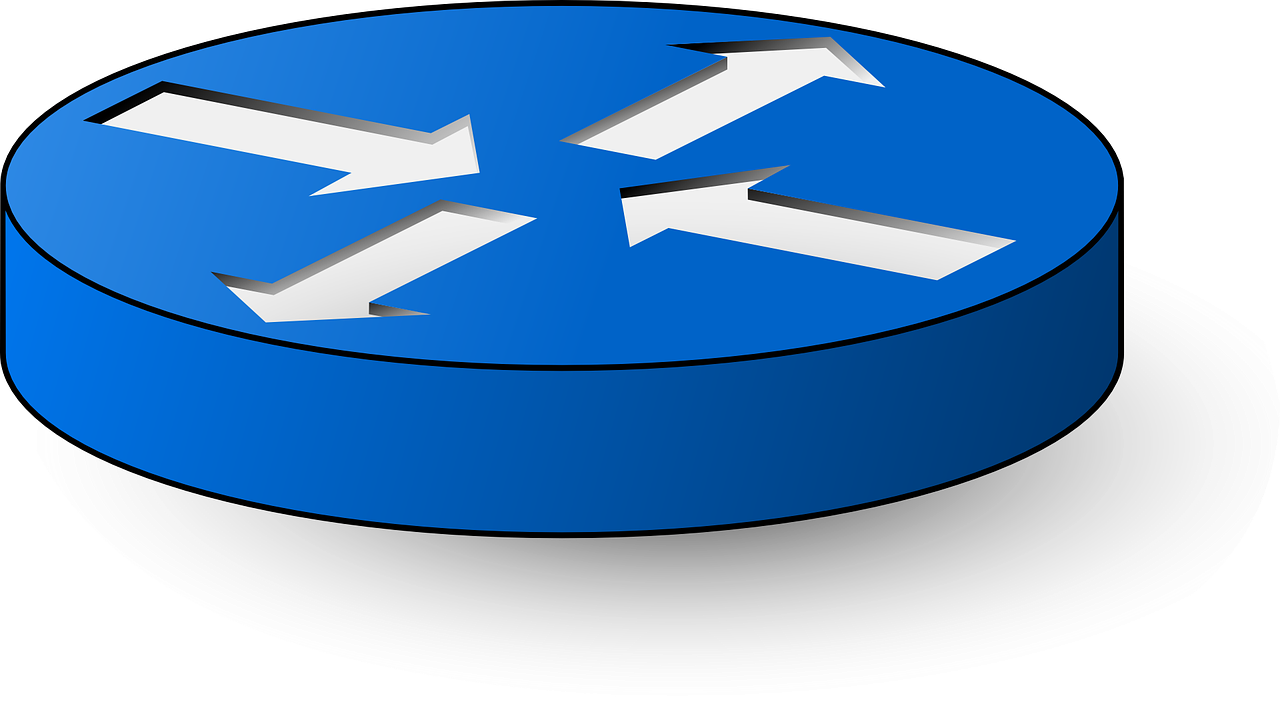
\includegraphics[width=52.5pt,height=52.5pt]{figures/router-30140_1280.png}};
%Image [id:dp8001089418713573] 
\draw (180,373.5) node  {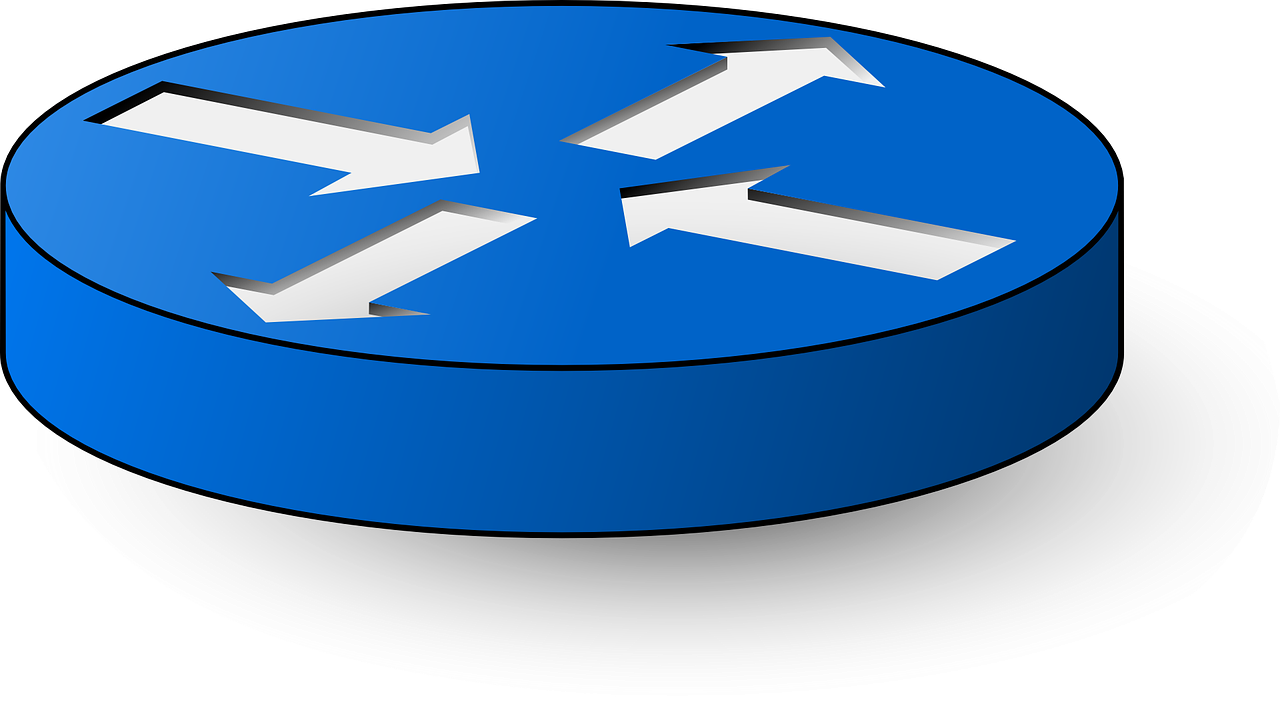
\includegraphics[width=52.5pt,height=52.5pt]{figures/router-30140_1280.png}};
%Image [id:dp9285996053263255] 
\draw (220,310.5) node  {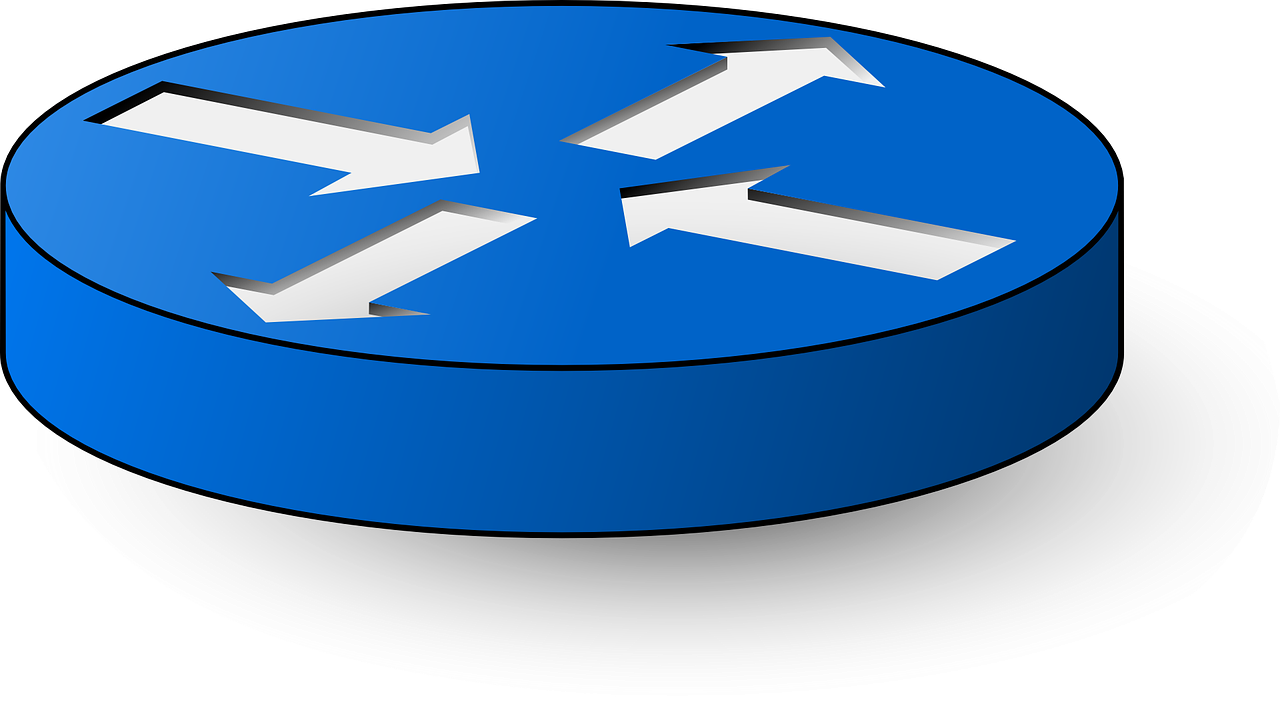
\includegraphics[width=52.5pt,height=52.5pt]{figures/router-30140_1280.png}};
%Image [id:dp3146785253004203] 
\draw (406,324.5) node  {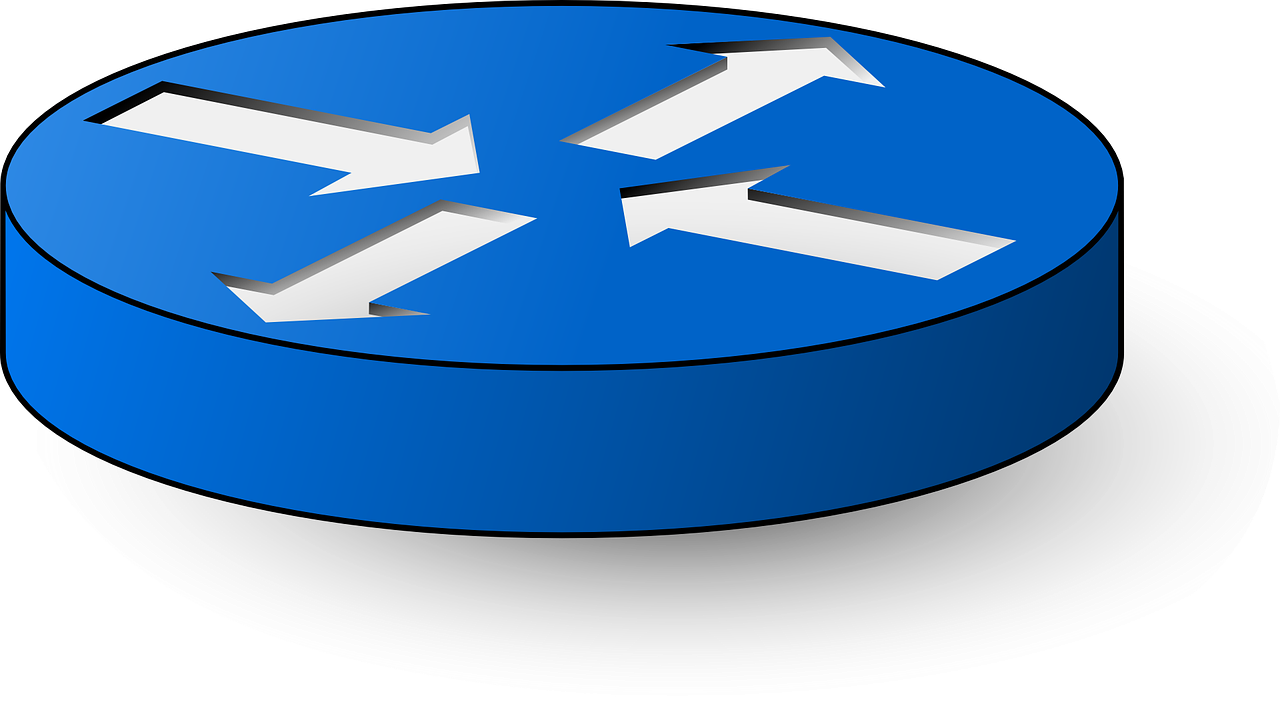
\includegraphics[width=52.5pt,height=52.5pt]{figures/router-30140_1280.png}};
%Image [id:dp3289010965024106] 
\draw (535,313.5) node  {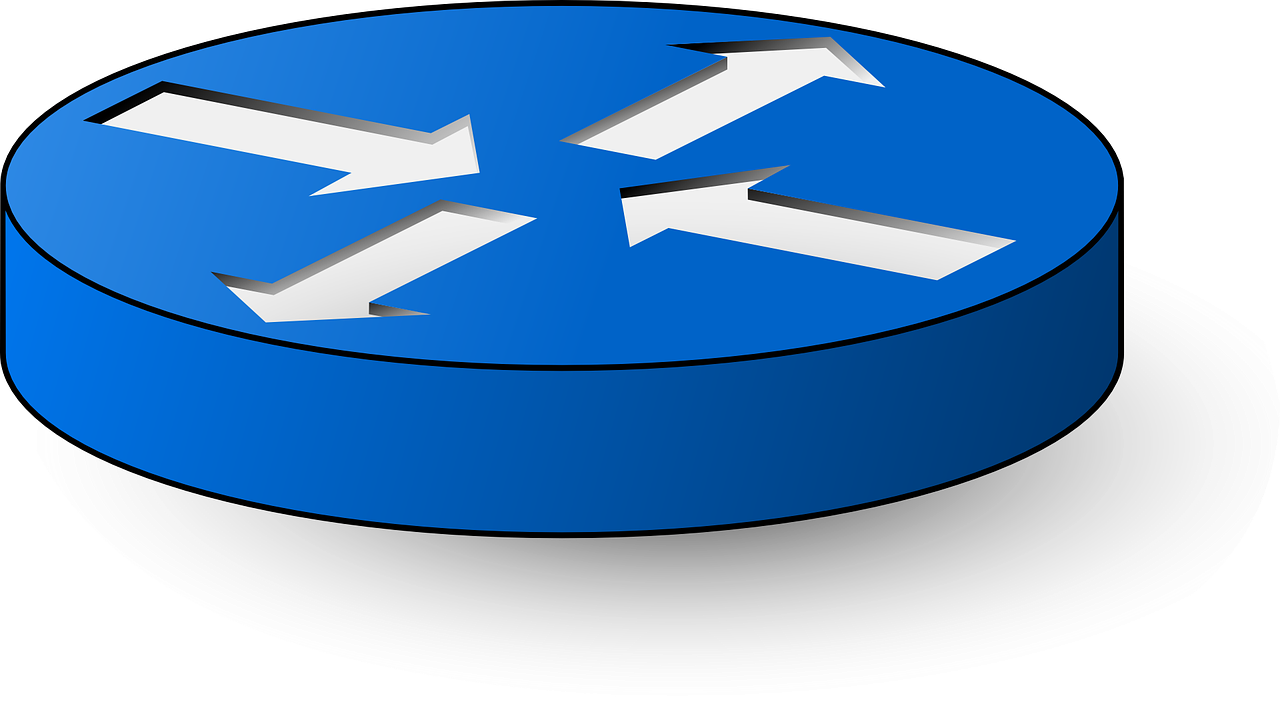
\includegraphics[width=52.5pt,height=52.5pt]{figures/router-30140_1280.png}};
%Image [id:dp13463717449619406] 
\draw (535,386.5) node  {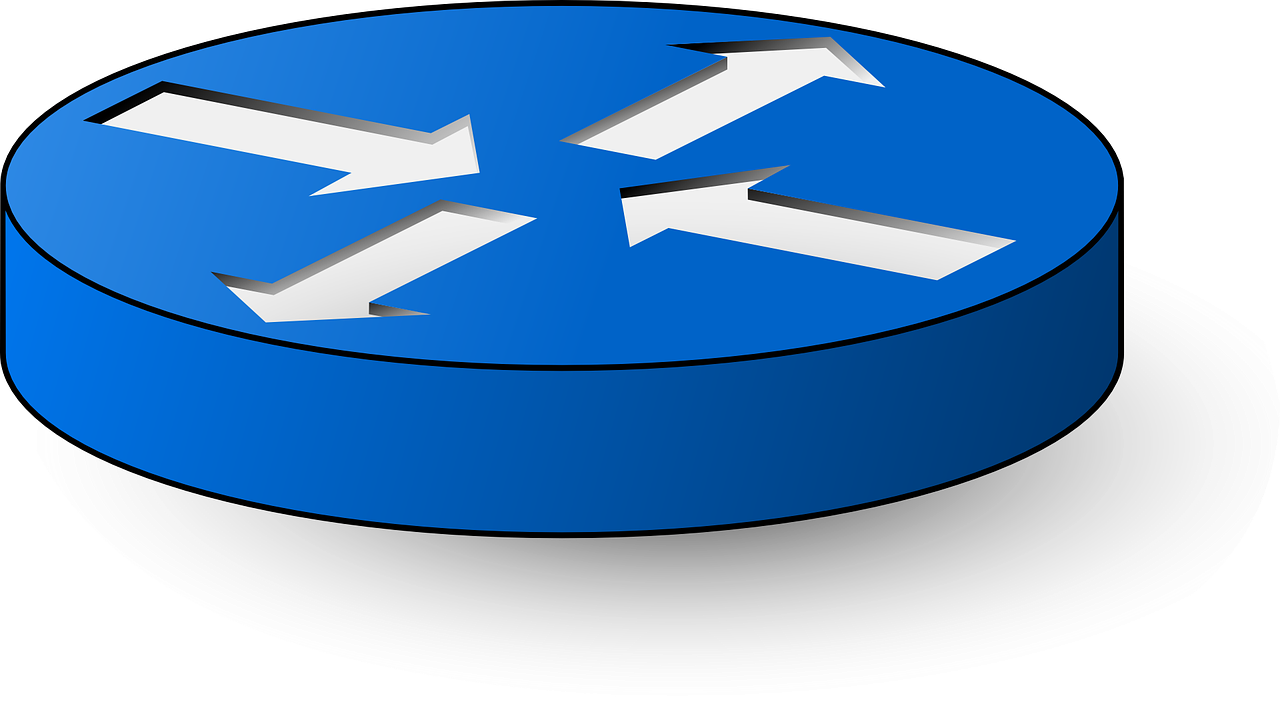
\includegraphics[width=52.5pt,height=52.5pt]{figures/router-30140_1280.png}};
%Straight Lines [id:da2794186668497024] 
\draw [line width=1.5]  [dash pattern={on 1.69pt off 2.76pt}]  (83,177.17) -- (82,307.97) ;


%Straight Lines [id:da3468403679668073] 
\draw [line width=1.5]  [dash pattern={on 1.69pt off 2.76pt}]  (158,228.17) -- (160,341.97) ;


%Straight Lines [id:da6099923036688548] 
\draw [line width=1.5]  [dash pattern={on 1.69pt off 2.76pt}]  (196,123.17) -- (197.2,280.27) ;


%Straight Lines [id:da9880025849572002] 
\draw [line width=1.5]  [dash pattern={on 1.69pt off 2.76pt}]  (318,140.17) -- (235.6,279.47) ;


%Straight Lines [id:da6145453947319308] 
\draw [line width=1.5]  [dash pattern={on 1.69pt off 2.76pt}]  (516,141.17) -- (515.6,283.07) ;


%Straight Lines [id:da41673177695849406] 
\draw [line width=1.5]  [dash pattern={on 1.69pt off 2.76pt}]  (413,143.17) -- (410.4,290.27) ;



% Text Node
\draw (105,397.5) node [scale=0.9] [align=left] {Physical Infrastructure};
% Text Node
\draw (89,74.5) node  [align=left] {{\small vSDN1}};
% Text Node
\draw (327,70.5) node [scale=0.9] [align=left] {{\small vSDN2}};


\end{tikzpicture}}


\caption{Principle of Virtual Network Embedding.}
\label{fig:VNE}
\end{figure}

\paragraph{Virtual Network Embedding Component}

The Virtual Network Embedding Component (VNEC) is in charge of determining the optimal set of physical resources to embed a virtual network and to handle the case where a virtual network must be migrated due to failure of a switch or because of an attack on the system.

\subparagraph{Virtual Network Embedding}
The Virtual Network Embedding (VNE) is a resource allocation problem, linked with Linear Programming and optimization techniques.
The use of VNE algorithm to automatically deploy virtual networks is compulsory to avoid manual and impractical configuration operations.
The VNEC is in charged of keeping track of available resources so he can determine whether or not to accept the virtual network creation request.
The set of physical resources may also be subject to location or security constraints.
A standard user requirements can be either resources or placement.
For instance, a user will need a certain amount of nodes, connected with a minimum bandwidth with the possibility to automatically migrate the topology in case of failures.
More specific constraints would be the physical location of the topology.
It can happen the traffic may not go through certain physical nodes.
This placement problem is similar to virtual machine placement since there might be legal limitations to ensure the data is staying in a closed environment.
Distributed network hypervisors or multi-cloud hypervisor may be subject to this constraint since network equipments are geographically distributed.
Security constraints include the availability of cryptography to cipher the communication end to end, the possibility to refuse to host a virtual network on the same physical substrate or even the same datacenter that another virtual network etc.

\subparagraph{Virtual Network Migration}
In order to answer to failures, attacks, and optimization issues, it is possible to migrate the virtual network on a different set of physical resources. 
Therefore, changes in the infrastructure, failure on a link or a switch, or over-consumption of network resources may require a change in the mapping of the virtual topology on the physical network.
The VNEC will be notified by the monitoring component, and then recompute the mapping of the topology with the physical infrastructure~\cite{VeRTIGO-Corin2012a,AutoSlice-Bozakov2012,CoVisor-Jin2015}.
There are cases where the tenant should be notified about the migration.
For instance, depending on the Service Level Agreement (SLA) between a particular tenant and the infrastructure provider, the migration may not be doable.

\paragraph{Resource Isolation}
The resource isolation component (RIC) ensures tenants that they are served the amount of resources they have requested.
It ensures that each tenant does not exceed the amount of resources they have been allocated.
FlowVisor-based hypervisors~\cite{FlowVisor-Sherwood2009,ADVisor-Salvadori2012,VeRTIGO-Corin2012a,EnhancedFV-Min2012,SlicesIsolator-El-Azzab2011,DoubleFV-Yin2013} all implement bandwidth and CPU isolation, and some tackle advanced issue on resource sharing. One of the problems with implementing resource isolation is that the hypervisor relies on vendor specific implementation of these isolation features, thus leading to heterogeneity problems.


\paragraph{Monitoring}
Monitoring the virtualization infrastructure serve two different purposes.
The first one is to ensure the proper functioning of the hypervisor's operations and is implemented on every hypervisor. However, it can range from switch discovery (similarly to a SDN controller) to resource monitoring and failure detection.
The second one is to serve the Security Component with data that will be used in detecting, preventing and mitigating attacks on tenants' virtual networks or on the hypervisor.
Most hypervisors implement a monitoring component to perform standard virtualization operations, while very few solutions implemented a monitoring to support advanced features or detect attacks~\cite{VeRTIGO-Corin2012a,CoVisor-Jin2015,FlowN-Drutskoy2012,AutoSlice-Bozakov2012,NVP-Koponen2014,ONVisor-Han2018}.

There are several different type of information hat must be monitored:

\subparagraph{Tenant to hypervisor traffic} Requests and configuration commands sent by a tenant can impact the security of the virtualization infrastructure. A malicious tenant may exploit vulnerable hypervisors by sending forged requests that will alter legitmate users' virtual networks. The monitoring module may forward the tenant's requests to the Security Component for further investigation.

\subparagraph{Management traffic} 
The notifications sent by topology discovery protocols such as LLDP notify the hypervisor about the current state of the physical network equipments. If a switch has a failure or becomes the target of an attack the VNEC or the Security Component will be notified. The VNEC may then trigger a migration to relocate the virtual network on a new physical substrate or the Security Component will raise an alert and trigger mitigation procedures.
Management traffic also includes packets sent by and to physical equipments to ensure their proper functioning.
This includes metrics about the resources used on each switch, information about the particular configuration of a switch or the potential errors raised.

\subparagraph{Configuration requests} An attacker located inside the physical infrastructure may leverage vulnerabilities in switches or in the authentication scheme to deploy malicious configuration rules These rules may alter the behavior of the networking equipments and may lead to a data exfiltration scenario or a Denial of Service.
The Security Component will be notified about these configuration packets.

\paragraph{Security Component}
The Security Component (SC) is in charge of detecting, preventing and mitigating attacks on the virtualization infrastructure. The SC relies on the monitoring in the infrastructure to collect useful data related to the security of the virtual networks and the physical equipments.
The problem of the security inside a network hypervisor is not very well studied and especially in the context of the migration of virtual networks.
The SC can operate on several levels, namely detection, prevention and mitigation.

\subparagraph{Detection}
The detection of attacks relies on associating networking events and tenant inputs with a security model.
For instance, the number of tenant requests may be monitored in order to detect a flooding behavior that would lead to an overload of the system. Another fitting example is to examine the content of configuration rules and determine if their deployment in the infrastructure would generate unwanted behavior.
There is so far no proposition of an attack detection mechanism for network hypervisors.

\subparagraph{Prevention}
Prevention of attacks can be implemented by either limiting the attack surface accessible to an attacker or by preventing the attack to reach its destination. The limitation of the attack surface is proposed by CoVisor~\cite{CoVisor-Jin2015} where each tenant is limited in its ability to process packet.
NVP~\cite{NVP-Koponen2014} implements tunnels between virtual nodes to simplify the routing the physical infrastructure and ensure a certain level of confidentiality.
ONVisor~\cite{ONVisor-Han2018} implements an access control module in charge of authenticating tenants applications and prevent them from interfering with other virtual networks.
This will require the setup of particular pipeline that may redirect packets to the security component and drop them accordingly. This aspect is not well exploited because it is strongly correlated to the ability of detecting attacks, which is also not well investigated. 

\subparagraph{Mitigation}
Depending on the type of attack, the mitigation can take several form. 
In case of a DoS attack, the security component would rely on the VNEC to provide an adequate migration scheme but it can also improve the performance of the VNEC by leveraging security techniques to determine a better substrate. 
If the configuration of physical nodes has been altered, the redeployment of configuration rules could take into account the location of the attacker.


% \paragraph{Workflows}
% In this section, we describe how the different components interacts together.
% There are several scenarios presented, initial deployment, migration.
% %\FC{Add scenarios if needed}
% Figure~\ref{fig:Workflow} represents the interactions and interfaces of these processes.
% \subparagraph{\textbf{Initial Deployment}}\textbf{}\\
% In a first time, the tenant will use the configuration component to describe the topology and the resources needed, as well as the different authorizations for communicating with other tenants' topologies.
% The output of this component would be a configuration file.
% Then, this file will be transmitted to the abstraction component (AC), the multi-tenants communication component (MCC) and the VNE Component.
% There are three simultaneous steps.
% The abstraction component will store the resources requested by the users.
% The MCC will store the description of the rights given by the user to the other tenants.
% The configuration file will be analyzed by the VNE component in correlation with the MCC and  the AC and will decide, if possible, which physical nodes are best suited to host this topology, according to the resource allocation policy.
% At this point, the hypervisor knows which nodes and which links will be used for this topology.
% The mapping computed by the VNE will be stored in the AC so it can process user requests.
% Therefore, these information can be transmitted to the VNI component that will push the different flow rules into the nodes.
% However, in case the requested topology cannot fit in the infrastructure, due to lack of resources, inter-tenants communication requests etc., the VNE component must return an error to the user.

% \begin{figure}[h]
% \centering
% 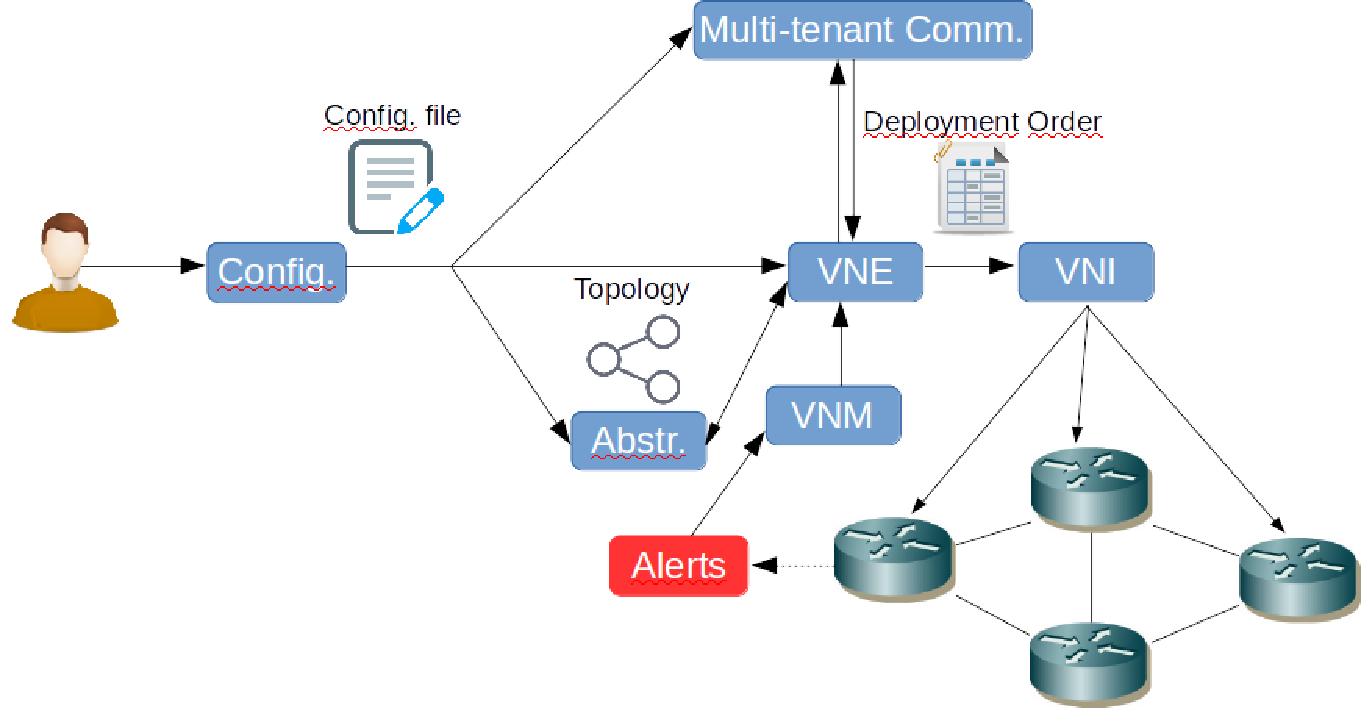
\includegraphics[scale=0.7]{figures/network-hypervisor-workflow}
% \caption{Deploying a topology in a network hypervisor.\label{fig:Workflow}}
% \end{figure}

% \subparagraph{\textbf{Migration}}\textbf{}\\
% The migration component collects alerts from the infrastructure about failures or resource congestion.
% Figure~\ref{fig:Workflow} illustrates how the component receives an infrastructure alert and transmits it to the VNE component so he can recompute the topologies.

% During runtime, a user may push a request for resources.
% This request is transmitted to the RAC for verification.
% If the request can be granted, the RAC will notify the VNI to deploy the resources.
% Oherwise, an error should be raised and returned to the user.